\chapter{Geothermal Background}\label{ch2:background}
\section{Geothermal Systems}\label{ch2:geosys}
\subsection{Origins of Heat}\label{ch2:heatorig}
\subsubsection{Accretion}\label{ch2:accrete}
The story of geothermal energy begins with the birth of planet Earth. Approximately 4.56 billion years ago \citep{allegre_age_1995, patterson_age_1956}, the Earth coalesced as a molten body heated by repeated impacts with other objects in the early solar system, like the planetesimal collision responsible for the formation of the Moon \citep{stevenson_origin_2014}. Over tens of millions of years, the Earth compacted, cooled, and differentiated, settling into the now familiar layered structure of a solid inner core, liquid outer core, viscous mantle, and outermost brittle crust \citep[p.\ 7]{press_understanding_2004} (Figure \ref{fig:earth_structure}). The intense heat from that early accretionary history remains concentrated in the core, where temperatures --- a matter of continued debate --- fall in the range of $6000\pm500$~K \citep[p.\ 372]{fowler_solid_2005}. Of the heat reaching the surface of the earth, $\approx 60\%$ flows through conductive and convective pathways from the lower crust or below \citep{stein_heat_1995}. Diffuse conductive heat transfer occurs everywhere across the Earth’s surface, but narrow zones of high heat flow follow crustal plate boundaries. In fact, the subduction-sourced volcanoes that ring the Pacific Ocean, divergent zones at the mid-ocean ridges and East African rift, and major strike-slip boundaries like the San Andreas fault zone all mark locations where focused heat anomalies are being tapped by geothermal installations \citep[p.\ 16]{dipippo_geothermal_2012}.

\begin{figure}[!htp]
\centering
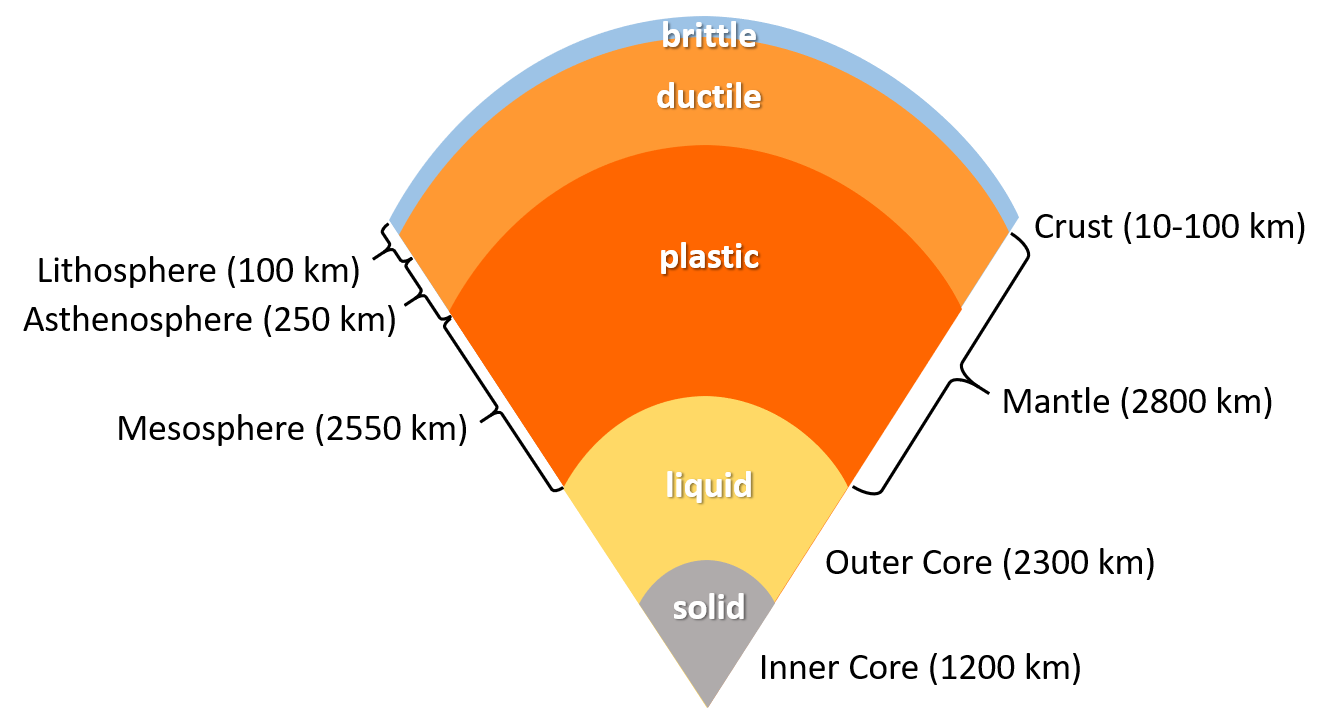
\includegraphics[width=.9\textwidth]{templates/images/Figure-Earth_structure.png}
\caption[Earth mechanical and compositional structure]{Inner structure of planet Earth by mechanical properties (left) and composition (right). Approximate layer thicknesses are noted in parentheses.}
\label{fig:earth_structure}
\end{figure}

\subsubsection{Radioactive Decay}\label{ch2:radio}
The second major source of heat within the Earth is the decay of radioactive isotopes. Early radioactive heating included radioisotopes with short half-lives like Aluminum-26 and Hafnium-182, which are now no longer present \citep[p.\ 16]{glassley_geothermal_2015}. Among the radioactive elements most influential to crustal heat  today are uranium (U), thorium (Th), rubidium (Rb), and potassium (K) \citep[p.\ 17]{glassley_geothermal_2015}. The decay of these and other elements accounts for 40\% of the crustal thermal budget \citep{stein_heat_1995}. But element abundances are not distributed uniformly throughout the crust. On average, continental crust, particularly the upper continental crust, has significantly higher concentrations of U, Th, and K radioactive elements compared to oceanic crust, and both types of crust are 1--2 orders of magnitude more enriched than the mantle \citep[p.\ 276]{fowler_solid_2005}. This relationship holds for representative igneous rock types; granite generates more heat than basalt, and both out-produce ultramafic rocks like peridotites \citep[p.\ 276]{fowler_solid_2005}.
%Present day heat flux estimates for the whole Earth amount to 87 mW/m$^2$ \citep{stein_heat_1995}. 

\subsection{Measuring Heat}\label{ch2:heat_measure}
\subsubsection{Geothermal Gradient}\label{ch2:geotherm}
Subsurface conditions show an increase in temperature with depth sustained by the flow of original accretionary heat and generated radioactive heat. This is commonly referred to as the geothermal gradient and averages $\approx30$ K%C
/km for continental crust \citep[p.\ 209]{press_understanding_2004}. Horizontal thermal gradients exist and can be quite high (e.g., at the contact between country rock and intruded magma), but they are assumed to average 0 K/km globally. Deviations from the average geothermal gradient are common and reflect the complexity of the rock record. The crust comprises distinct layers, or strata, that vary in composition and rock type. Unlike igneous formations that can be relatively homogeneous, sedimentary rocks derive from surface processes that mix sediments from a variety of original source rocks with different degrees of sorting \citep[p.\ 164--168]{press_understanding_2004}. Alteration from fluids, heat, and pressure can then modify the composition of these rocks, causing constituent minerals to change form and arrangement to create metamorphic rocks \citep[p.\ 195--205]{press_understanding_2004}. The spatial and depth variations in these formations, enhanced by structure processes like faulting, create subsurface compositional heterogeneity, directly reflected in rock properties. Thermal conductivity, specifically the ability to move deep-sourced heat to shallower depths, and radioactive element abundance, or the ability to generate additional heat in situ, can therefore vary in all directions in the subsurface. Thermal heterogeneity can be further compounded by anomalies created from salt movement \citep[p.\ 164--168]{press_understanding_2004}, magmatic intrusions, or global tectonic processes. Geology and geologic history therefore play an important role in defining the geothermal gradient of an area.

\subsubsection{Heat Flow}\label{ch2:heatflow}
Fundamentally, heat moves in the direction from hot to cold (Second Law of Thermodynamics) at a rate that linearly scales with the thermal gradient. Simple one-dimensional thermal conduction can be characterized by the relationship \citep[Fourier's Law,][p.\ 270]{fowler_solid_2005}:
\begin{equation}\label{eq:conduction}
    {\bf q} = -k\nabla T
\end{equation}
where ${\bf q}$ is heat flux, or heat flow per unit time per unit area, with S.I.\ units of W$\cdot$m$^{-2}$. Heat flux depends on the gradient of temperature ($T$) and the thermal conductivity ($k$), that is, the ability of material to conduct heat. Different rock types have different values of $k$, e.g., sandstone varies from 1.60--2.10 W/m$\cdot$K, granite has higher values of 1.73--3.98 W/m$\cdot$K \citep[p.\ 30]{dipippo_geothermal_2012}. The most abundant minerals in crustal rocks, feldspars and quartz, can differ in $k$ values by up to 3 $\times$ in value, so their relative fractions strongly influence the thermal conductivity of a formation \citep[p.\ 22]{glassley_geothermal_2015}. Regardless, these and other common crustal minerals tend to be poor thermal conductors compared to metals like aluminum (210 W/m$\cdot$K) and iron (73 W/m$\cdot$K), making crustal conduction a slow means of heat transfer \citep[p.\ 23]{dipippo_geothermal_2012}.

Conduction dominates on local scales in the crust, while convection is the primary means of heat transfer on global, tectonic scales. Even in its two-dimensional form with no internal heat generation, the equation governing convection is much more complex than for conduction \citep[p.\ 267]{turcotte_geodynamics_2002}:
\begin{equation}\label{eq:convection}
\frac{\partial T}{\partial t} = \frac{1}{\rho c_P}\nabla\bullet\left(k\nabla T\right)-{\bf u}\bullet\nabla T
\end{equation}
where \textbf{u} is the velocity of the fluid, $\rho$ is the material density, and $c_P$ is the specific heat, which defines the amount of heat necessary to raise 1 kg of that material by $1$ K. Convection combines heat transfer from conduction with mass movement. Since mantle minerals are poor conductors of heat, the mantle insulates and traps heat from the core near the core-mantle boundary \citep[p.\ 25]{glassley_geothermal_2015}. The combined effects of lower viscosity, thermal expansion, and buoyancy forces near that boundary all drive convective mantle flow \citep[p.\ 25]{glassley_geothermal_2015}. Mantle convection is responsible for the high heat-flow values at crustal plate boundaries like mid-ocean ridges, as well as intraplate hot spots underlying Hawaii, Yellowstone, and several other locations around the world. Smaller-scale convection also takes place at subduction zones where the water-rich material from the down-diving plate experiences low-temperature melting, migrates upwards, and forms volcanic arcs on the surface as observed in Japan, Indonesia, and the U.S.\ Pacific Northwest \citep[p.\ 31-33]{press_understanding_2004} --– all locations with geothermal potential.

Heat-flow measurements capture the flux of heat through the Earth’s surface as a result of these and other complex subsurface processes. In this respect, heat flow serves as a simpler, more accessible geothermal metric than the more sparsely-measured geothermal gradient. Today, high-quality heat flow measurements can be obtained in marine conditions, along continental margins, on mid-ocean ridges, and from the multitude of wells drilled by the oil \& gas industry, supporting large aggregate data sets like the New Global Heat Flow Database \citep{lucazeau_analysis_2019}. As Figure \ref{fig:heatflow} shows, data from these collections can be gridded to create spectacular maps of heat flow variations around the world. These maps offer a good starting point for quickly targeting regional-scale geothermal potential, which can be further refined through other methods (see Section \ref{ch2:geoexp}).

\begin{figure}
\centering
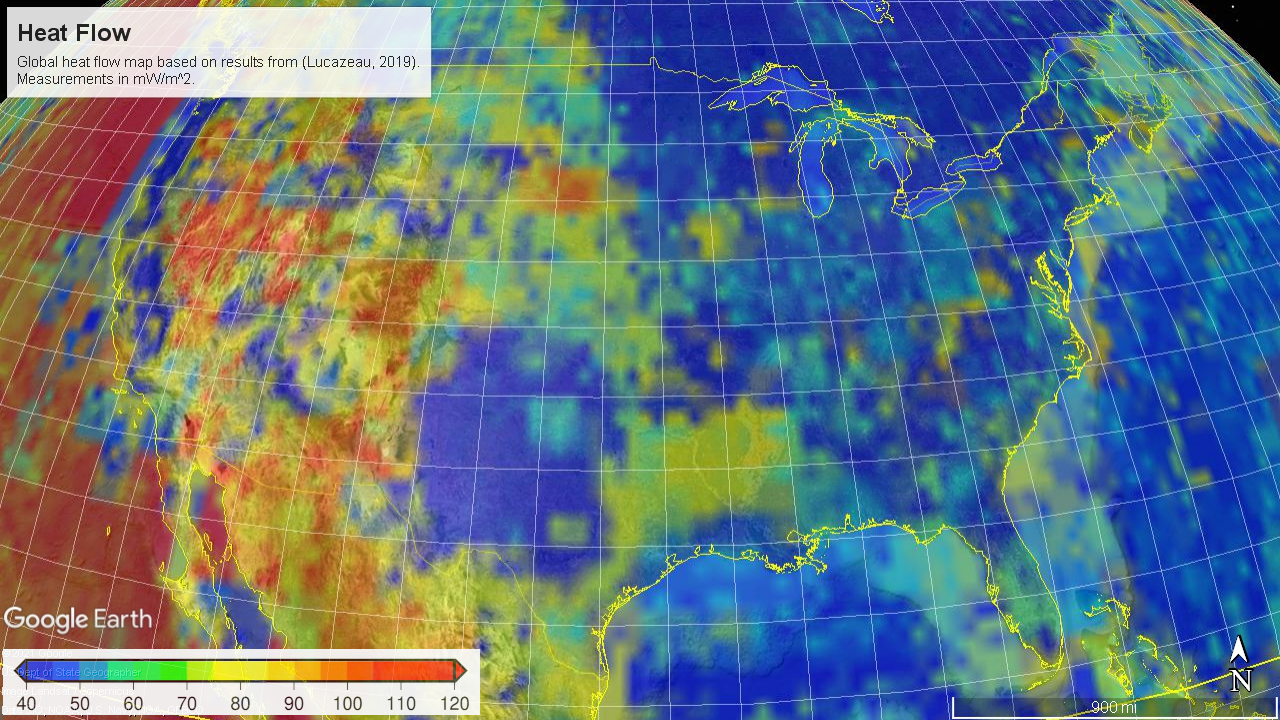
\includegraphics[scale=0.45]{Figure-HeatFlowMap}
\caption[Heat flow across the continental U.S.]{Heat flow estimates for the continental United States, plotted in Google Earth with data layer from \protect\citep{lucazeau_analysis_2019}.Units are mW/m$^2$.}
\label{fig:heatflow}
\end{figure}

\subsection{System Fundamentals}\label{ch2:sysfund}

The conventional concept of a geothermal system consists of five key entities \citep[p.\ 9]{dipippo_geothermal_2012}:
\begin{enumerate}[itemsep=2pt] \label{list:sysreq}
   \renewcommand{\labelenumi}{\roman{enumi}}
   \item Heat source of significant size and temperature
   \item Permeability, typically in the form of a fracture network within crystalline rock
   \item Ample volume of working fluids e.g., water from precipitation and drainage
   \item An impermeable sealing layer
   \item Consistent, reliable fluid recharge
\end{enumerate}

\subsubsection{Hydrothermal Systems}\label{ch2:hydro}

If naturally present, the combination of these five elements defines a hydrothermal system. As water percolates down, captures heat from the permeable thermal reservoir, and gets trapped beneath the sealing caprock, a small fraction of the resource can escape to the surface to produce distinctive geothermal manifestations like fumaroles, hot pools, geysers, mud pots, and discolored or altered rocks (Figures \ref{fig:lassen-geysers} and \ref{fig:lassen-mudpot}). These features are strong indicators of hydrothermal activity at depth.

\begin{figure}
\centering
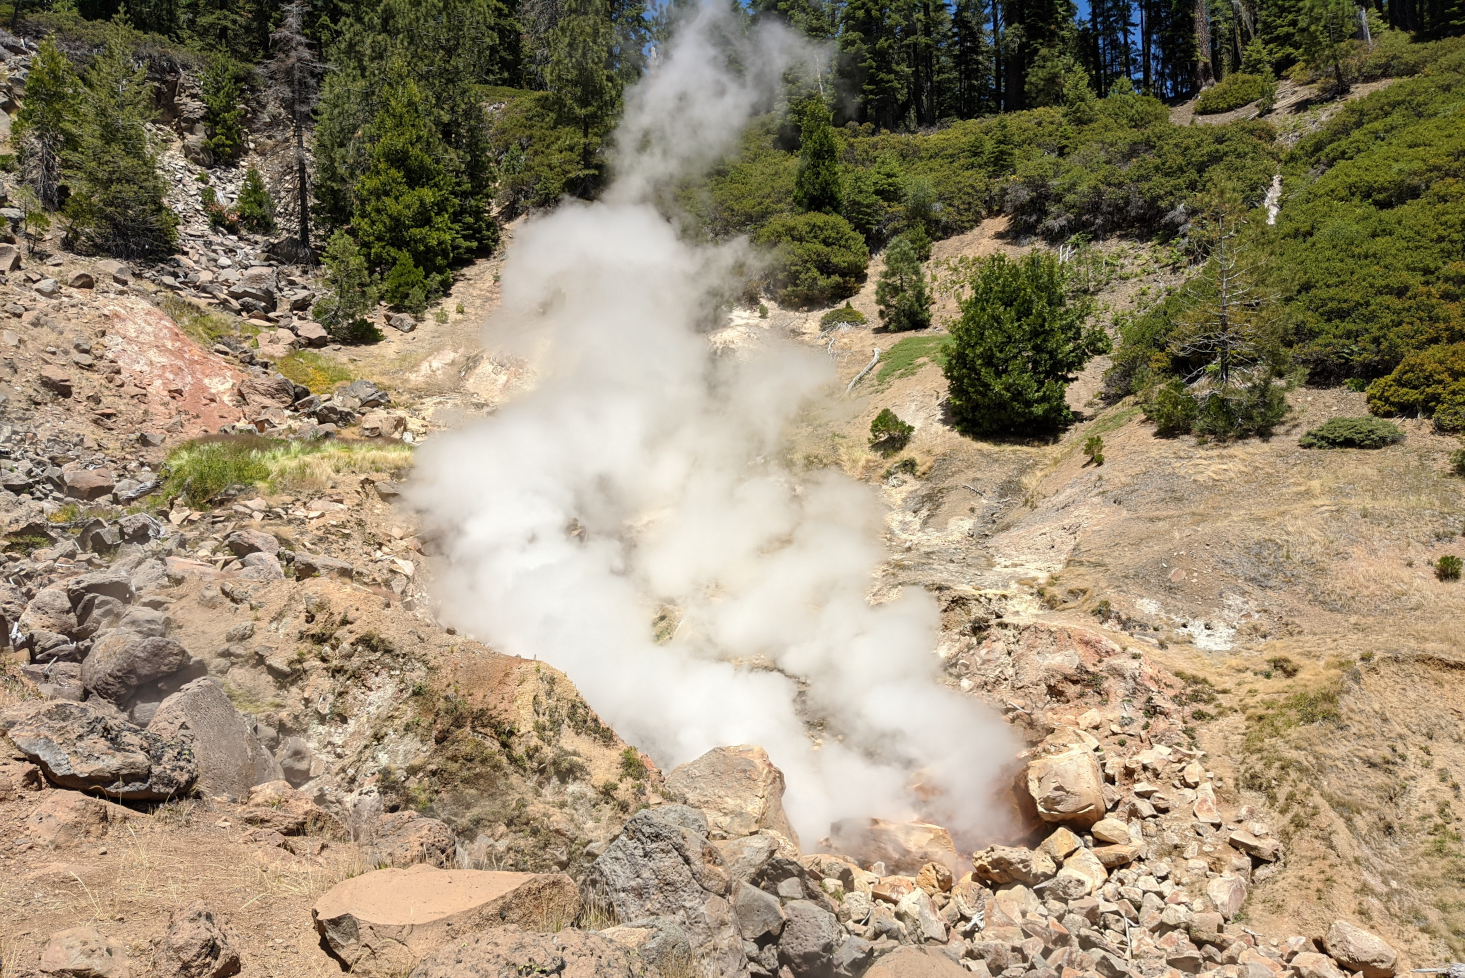
\includegraphics[width=0.8\linewidth]{Figure-Lassen-geysers3}
\caption[Terminal Geyser, Lassen National Park]{Terminal Geyser, Lassen National Park, California. Photo credit: Author}
\label{fig:lassen-geysers}
\end{figure}

\begin{figure}
\centering
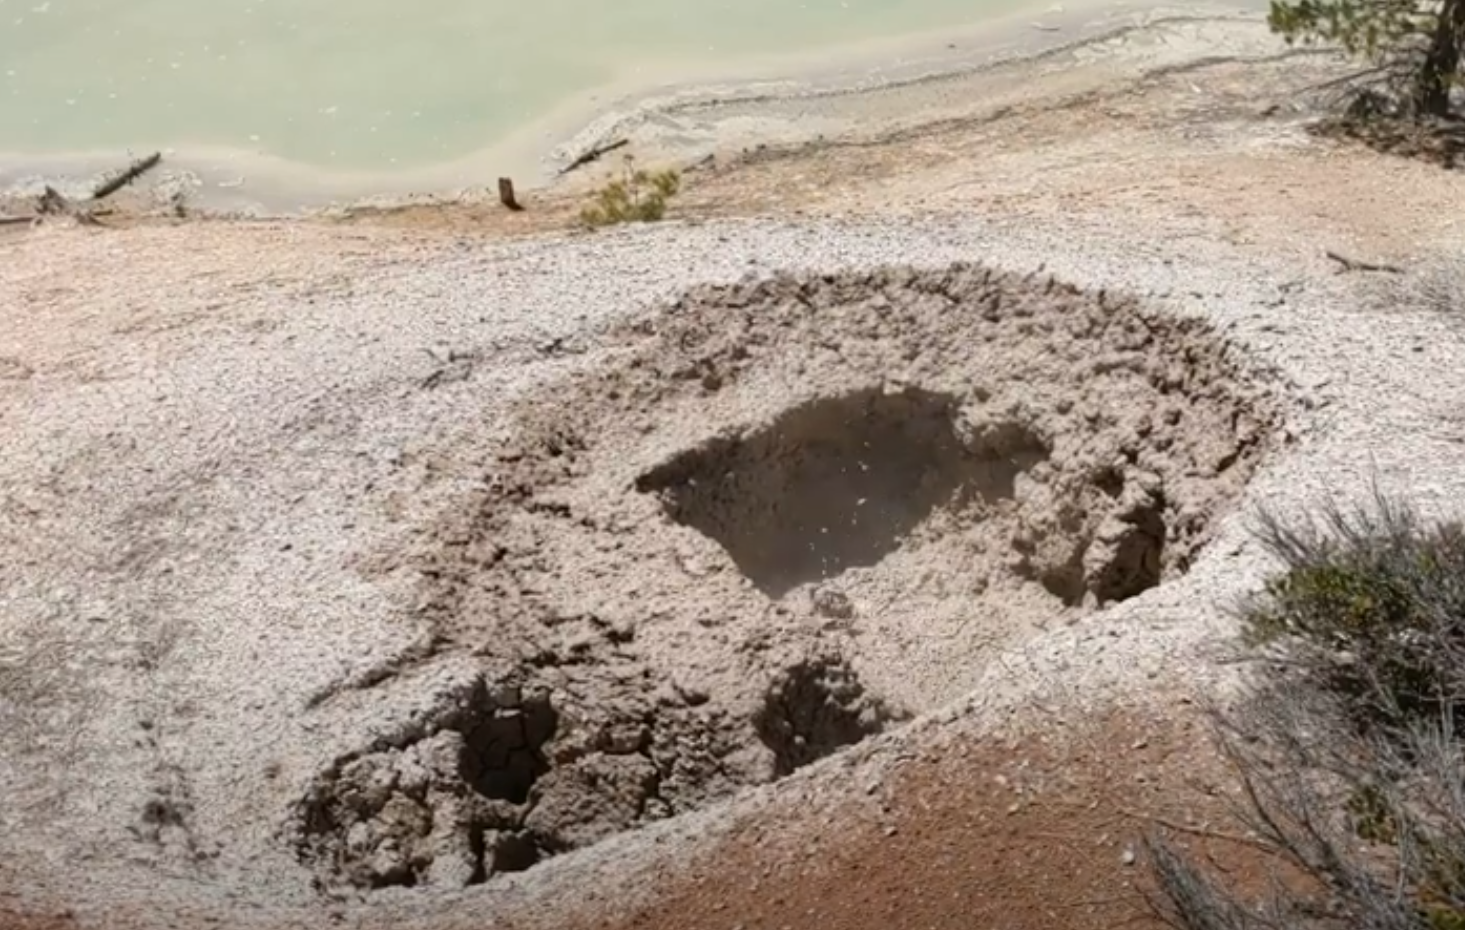
\includegraphics[width=0.8\linewidth]{Figure-Lassen-mudpot}
\caption[Mud pot, Lassen National Park]{Active mud pot and ground staining on the bank of Boiling Springs Lake, Lassen National Park, California. Photo credit: Author}
\label{fig:lassen-mudpot}
\end{figure}

Hydrothermal resources have been exploited by humans for many millennia. Artifacts show proto-Native American use of hydrothermal waters for cleaning and health restoration over 10,000 years ago \citep{doe_history_2021}. The importance of geothermal hot springs for Roman, Japanese, Chinese, and Ottoman baths is also well-established in the historical record \citep{lund_characteristics_2007}. Industrial use began in the 1800s with chemical extraction from geothermal steam, pools, and deposits in Larderello, Italy \citep[p.\ 251]{dipippo_geothermal_2012}. Geothermal district heating, or large-scale heating of residences and businesses using geothermal-produced fluids, was pioneered in Chaudes-Aigues, France in the 1300s and first introduced to the United States in 1892 with an installation in Boise, Idaho \citep{lund_characteristics_2007}.

These few examples show some of the many opportunities for low-temperature ($T<90^\circ$C) and medium-temperature ($90^\circ{\rm C}<T<150^\circ$C) geothermal resource use, which extends beyond just hydrothermal systems. District heating can help meet building and water temperature needs, and agriculture, textiles, chemicals, and even the food industry can benefit from access to low-temperature geothermal \citep{doe_low_2021, liu_overview_2015}. Growing interest has led to dedicated funding opportunities; the \acrlong{gto} (\acrshort{gto}) within the \acrlong{doe} (\acrshort{doe}) recently awarded a grant to Cornell University to pilot a deep direct-use geothermal project providing baseload heating for the university campus during cold New York winters \citep{hamm_geothermal_2021,tester_integrating_2015}.

The topic of this thesis instead concerns the use of moderate- to high-temperature geothermal for generating electricity. The first example of geothermal power production came from Italian experiments in 1904, and the first commercial plant went online in Larderello, Italy in 1914 \citep[p.\ 251]{dipippo_geothermal_2012}. Geothermal power made its debut in the United States with the development of The Geysers field beginning in 1960 \citep{tester_future_2006}. Hydrothermal plants quickly appeared in New Zealand, Japan, Iceland, Indonesia, Kenya, the Philippines and elsewhere throughout the 1970s-1980s, with continued growth through to present-day \citep{lund_characteristics_2007}. 2020 statistics from the International Renewable Energy Agency (IRENA) place the United States as world leader in geothermal installed capacity (2587 MW), followed by Indonesia (2131 MW), and the Philippines (1928 MW) \citep{irena_country_2021} (Figure \ref{fig:irena-rank}). 

\begin{figure}
\centering
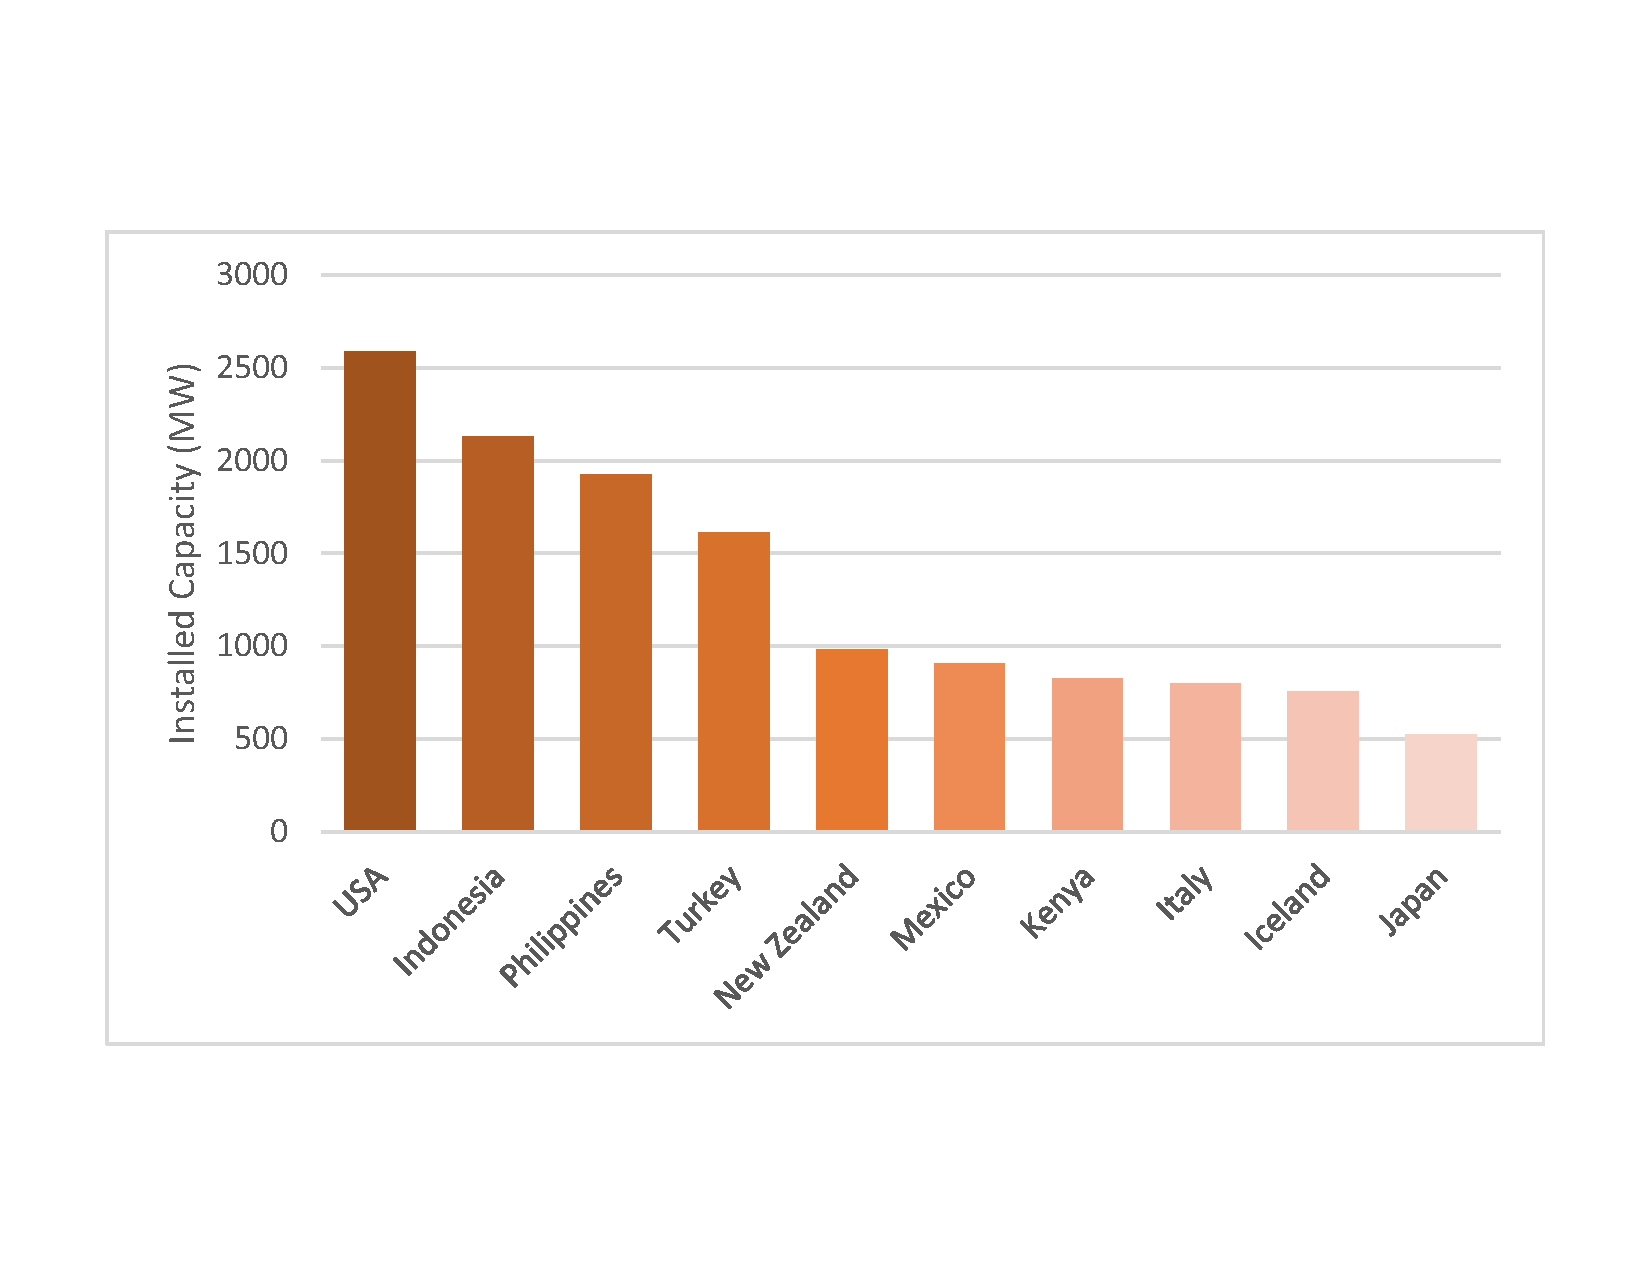
\includegraphics[width=.8\textwidth]{templates/images/Figure-IRENA_statistics.pdf}
\caption[Country rankings for installed geothermal capacity]{Countries ranked by installed geothermal capacity based on 2020 statistics, adapted from \protect\citep{irena_country_2021}}
\label{fig:irena-rank}
\end{figure}

A comprehensive assessment of moderate and high-temperature \acrlong{kgra}s (\acrshort{kgra}s) by the \acrlong{usgs} (\acrshort{usgs}) determined the U.S.\ has conventional geothermal (hydrothermal) power generation potential of $\approx9,000$ MW, and an additional $\approx30,000$ MW potential exists in undiscovered resources \citep{williams_assessment_2008}. The recent DOE GeoVision study notes hydrothermal potential in Alaska and Hawaii alone are $\approx8,000$ MW due to their unique tectonic environments (Aleutian subduction zone and Hawaiian hot spot, respectively), and high-case model estimates for the continental U.S.\ forecast an installed capacity of $\approx16.5$ GW by 2050 from known and unknown hydrothermal resources \citep{augustine_geovision_2019,hamm_overview_2019}.

\subsubsection{Enhanced Geothermal Systems}\label{ch2:egs}

Geothermal potential may even when one or more of the fundamental elements listed in Section \ref{ch2:sysfund} are missing. These unconventional geothermal systems, often referred to as \acrlong{egs} (\acrshort{egs}), contain a significant heat source but lack either the adequate permeability or sufficient rechargeable working fluids to meet the requirements of a hydrothermal system. A broader definition for EGS includes thermal production from sedimentary and crystalline tight rock, poorly-performing hydrothermal systems, co-production from oil \& gas operations, and even thermal recovery directly from magma \citep{tester_future_2006}. Focusing on the more common tight rock scenario, EGS systems work by artificially creating or improving reservoir permeability and ensuring sustained fluid flow through the reservoir \citep[p.\ 281]{glassley_geothermal_2015}. Fluids pumped down an injection well pass through a stimulated fracture network. Heat from the thermal reservoir warms the fluid before it returns to the surface via one or more producing wells and enters a power plant to produce electricity (Figure \ref{fig:egs_schematic}). Reservoir stimulation generally involves hydraulic fracturing or ``fracking” techniques to create pathways connecting injector-producer pairs. The technology and field capabilities are thus well-aligned with unconventional oil \& gas operations \citep{petty_synergies_2009}. 

\begin{figure}%[htp!]
\centering
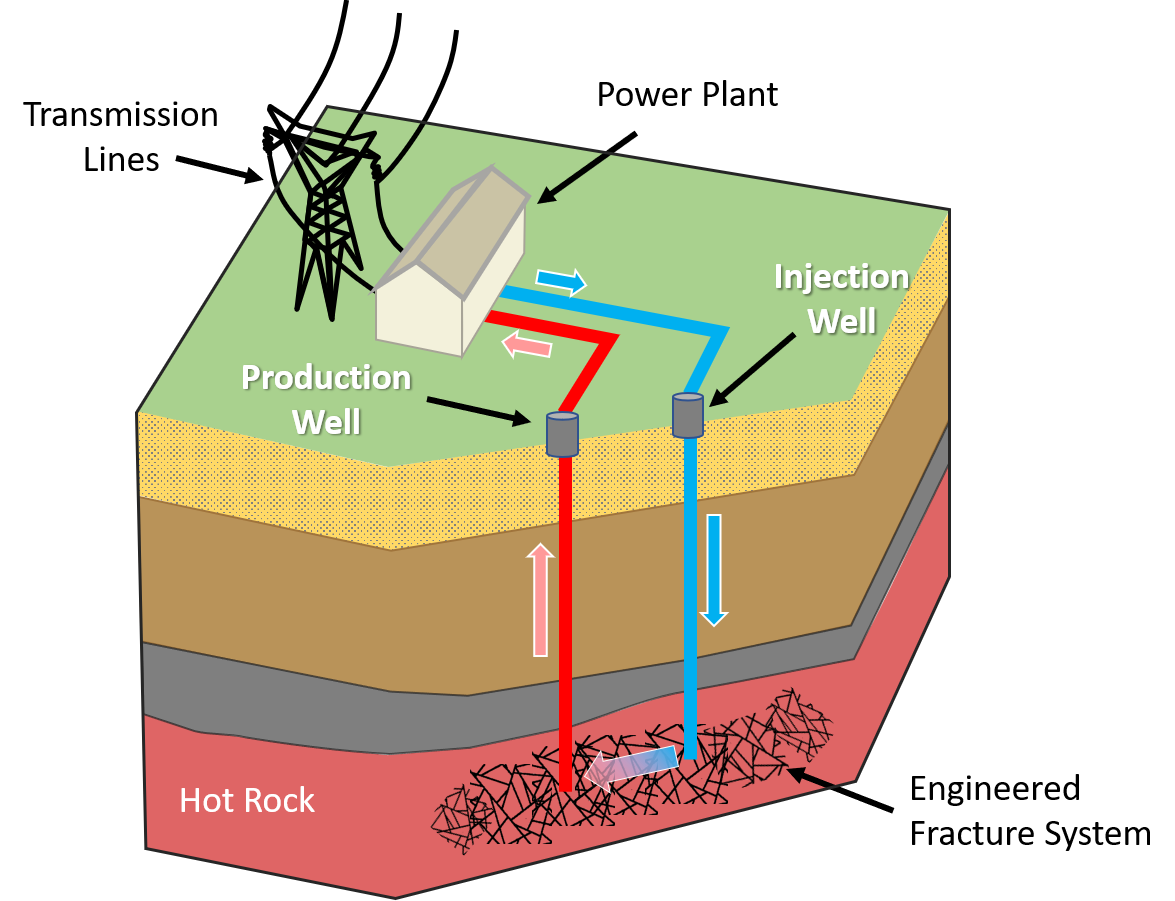
\includegraphics[width=.85\textwidth]{templates/images/Figure-EGS_Schematic.png}
\caption[EGS schematic]{Schematic diagram illustrating the EGS concept with a single injection-production well pair.}
\label{fig:egs_schematic}
\end{figure}

EGS could help propel geothermal beyond niche hydrothermal environments to become a more significant contributor to electricity production in the United States. The sources of subsurface heat exist everywhere (see Section \ref{ch2:heatorig}), so accessing temperatures that could support power production fundamentally rely on drilling deep enough and creating the artificial conditions necessary for heat capture. \acrlong{lanl} (\acrshort{lanl}) validated the EGS approach in crystalline rock at Fenton Hill beginning in 1974 \citep{tester_future_2006}. Feasibility studies followed soon thereafter in Japan, Germany, the U.K., and France \citep{breede_systematic_2013}. Among the most notable EGS projects providing key lessons learned are The Geysers (U.S.), Soultz-sous-Forêts (France), and Cooper Basin (Australia). The Geysers stands out as the largest geothermal power-generating complex in the world, delivering $\approx1,000$ MW even after 60 years of steam production \citep{jelacic_evaluation_2008,williams_assessment_2008}. Although drilling issues and public concern over induced seismicity halted efforts \citep{larson_altarock_2009}, rock-stimulation experiments in the NW Geysers proved distinct reservoirs can be developed adjacent to active hydrothermal operations \citep{pan_establishment_2019}. The Soultz project commenced in 1987 with one injector and two producers drilled to 5 km depth, eventually supporting a 1.5 MW power plant built in 2007-2008 \citep[p.\ 463]{dipippo_geothermal_2012}. In addition to experimental lessons learned for drilling, hydrofracturing, chemical stimulation, scaling, and corrosion, Soultz today supports both power production and district heating \citep{durst_overview_2013}. Cooper Basin, the largest EGS demonstration project of its time, showed great promise after a 6-year proof-of-concept phase \citep{stephens_assessing_2010}. However, the project halted in 2015 after a previously-unrecognized intersecting fault zone derailed further progress, highlighting the importance of robust structural appraisal in assessing geothermal prospects \citep{holl_what_2015}. 

As the fate of these projects might suggest, the long-standing promise of EGS has not yet been fully realized. However, several active projects supported by the \acrlong{nrel} (\acrshort{nrel}) and GTO (e.g., EDGE, EGS Collab, FORGE) are providing insights necessary to mature subsurface models, drilling technologies, and stimulation methods for more widespread EGS adoption \citep{hamm_geothermal_2021}. And recent technology advances and partnerships involving start-ups like Deep Earth Energy \citep{geoenergy_saskatchewan_2021}, Eavor Technologies \citep{ross_energy_2020}, Eden GeoTech \citep{daso_eden_2020}, and Fervo Energy \citep{moss_google_2021,shieber_geothermal_2021}, show there is a growing fervor to overcome technology roadblocks currently holding EGS back. Projections show the size of the prize with success in EGS. Assuming a maximum cut-off depth of 7 km and a minimum reservoir temperature of 150$^\circ$C, the EGS resource potential for electricity production in the continental United States might be at least 5,150 GW, with an additional $\approx1,500$ MW from Near Hydrothermal Field-EGS (\acrshort{nfegs}) \citep{augustine_geovision_2019}. To put this opportunity into context: the total utility-scale electricity generation capacity from \underline{all} sources in the United States was $\approx1,200$ GW in 2019, over 4$\times$ less in magnitude than predicted EGS potential \citep{eia_electric_2020}.
\vfill

\section{Geothermal Exploration}\label{ch2:geoexp}
\subsection{Background}\label{ch2:expl_background}
The identification of geothermal resources classically relied on surface expressions of hot fluids circulating at depth. Quite simply, if a bubbling hot spring or a geyser was present, you had a working geothermal system. Some of the first sites for geothermal power production, like Larderello and The Geysers, were (unsurprisingly) targeted because of their tell-tale surface characteristics \citep[p.\ 111]{glassley_geothermal_2015}. However, this prospecting method only applies to fully-functioning hydrothermal systems, and not all such systems have surface manifestations if fluids remain trapped beneath a subsurface impermeable seal. These hidden or “blind” geothermal resources require more sophisticated exploration methods to identify and assess accurately.

\subsection{Regional Exploration}\label{ch2:regional_expl}
Regional evaluation techniques historically depended on sparse borehole data to map the geothermal potential of the U.S.\ \citep{kehle_aapg_1970}. Successive efforts led to progressively more comprehensive collections of heat flow and bottom hole temperature (\acrshort{bht}) measurements \citep{blackwell_heat_1990, blackwell_temperature-at-depth_2011, muffler_assessment_1979, sorey_low-temperature_1983, wisian_heat_1999}, now widely-available with additional geothermal data through the DOE NGDS platform \citep{anderson_national_2013}. These efforts supported a better understanding of broad trends that tie directly to tectonic provinces in the United States. Subduction and transform plate boundaries to the West, combined with extension in the Basin and Range, make this area of the U.S.\ more susceptible to high heat flow, high geothermal gradients, and greater potential for hydrothermal activity \citep{mariner_low-temperature_1983}. Passive margins along the Atlantic and Gulf of Mexico sides of the country make those regions less likely to host significant hydrothermal systems, although surveys have identified sedimentary basins with elevated heat flow in the South (Louisiana-Arkansas), Central (Iowa-Illinois, Nebraska-South Dakota), and Eastern (Appalachians) United States \citep{blackwell_geothermal_1995, sorey_low-temperature_1983}.

\subsection{Sub-regional Exploration}\label{ch2:sub_regional_expl}
Continental maps provide a super-regional view of geothermal prospectivity, but further refinement is required to progress an exploration program. Specifically, the determination of regional plays and local prospects must come before deciding where and how to develop a geothermal field. Characterization activities can be decomposed into the evaluation of four earth subsystems: hydrologic, stratigraphic, structural, and thermal. The main types of surveys associated with each subsystem are listed in Table \ref{tab:survey_types} and discussed briefly in the following section. Note that survey methods typically provide information on multiple subsystems. The associated non-uniqueness of subsurface interpretations based on these surveys highlights the need to integrate multiple lines of evidence for exploration activities. 

\begin{table}
\begin{tabular}{ll}
\textbf{Hydrologic}     &                                                          \\ \hline
Earthquake records      & movement of magma or fluids                              \\
Geologic survey         & surface expressions (vents, geysers, deposits), drainage \\
Hydrologic survey       & fluid geochemistry, recharge and rate, water table       \\
Magnetic survey         & hydrothermal alteration                                  \\
Precipitation records   & water cycle inputs, recharge rate                        \\
Resistivity survey      & subsurface fluids or hydrothermal alteration             \\
Satellite survey        & surface drainage patterns, distribution of deposits      \\
Seismic survey          & presence and location of subsurface fluids               \\
                        &                                                          \\
\textbf{Stratigraphic}  &                                                          \\ \hline
Geologic survey         & stratigraphic successions, seal and reservoir             \\
Gravity survey          & density anomalies, stratigraphic variations              \\
Magnetic survey         & igneous formations, stratigraphy and reservoir           \\
Radiometric survey      & mineral abundances, source and reservoir                 \\
Resistivity survey      & thermal conductivity, lithology                          \\
Satellite survey        & distribution of outcrops and formations                  \\
Seismic survey          & stratigraphy and rock properties                         \\
                        &                                                          \\
\textbf{Structural}     & \textbf{}                                                \\ \hline
Aerial survey           & surface fault traces                                     \\
Earthquake records      & fault location, fault recency                                  \\
Geodetic survey         & active deformation or faulting                           \\
Geologic survey         & surface fault traces, fault recency                      \\
Gravity survey          & subsurface faults, plutons, salt                         \\
Resistivity survey      & fractured zones                                          \\
Satellite survey        & topography, structural patterns                          \\
Seismic survey          & subsurface faults, folds, other structural features      \\
                        &                                                          \\
\textbf{Thermal}        &                                                          \\ \hline
Aerial survey           & thermal anomalies in shallow subsurface (IR)             \\
Air Temperature records & near-surface thermal conditions                          \\
Geologic survey         & surface manifestations (dikes, vents, deposits)          \\
Gravity survey          & presence of high-T anomalies (e.g. magma)                \\
Hydrologic survey       & geothermometry, dominant geofluid liquid phase           \\
Radiometric survey      & radioactive heat generation                              \\
Resistivity survey      & thermal conductivity, temperature gradient               \\
Seismic survey          & depth to mantle, intrusive igneous features              \\
Temperature survey      & heat flow, geothermal gradient                          
\end{tabular}
\caption[Data-collection methods for geothermal subsystems]{Data collection methods useful for characterizing Earth subsystems that influence geothermal favorability.}
\label{tab:survey_types}
\end{table}

\subsubsection{Geologic Data Collection}\label{ch2:geologic_data}
Geologic field mapping can provide crucial direct evidence supporting the presence of geothermal systems. Surface manifestations like geysers, vents, and mud pots may also be coincident with mappable mineralogic indicators of the subsurface chemistry and style of geothermal activity. Volcanic-based geothermal systems tend to have acid-sulfate waters with hydrogen sulfide-rich brines that leave behind sulfur deposits \citep[p.\ 123]{glassley_geothermal_2015}. Bicarbonate geothermal waters can produce distinctive travertine terraces or subaqueous tufa deposits, as well as a unique variety of potassium feldspar called adularia \citep[p.\ 125]{glassley_geothermal_2015}. And chloride geothermal fluids are known to precipitate sinter or geyserite deposits composed of opal or amorphous silica \citep[p.\ 125]{glassley_geothermal_2015}. Elevated abundances of trace elements like boron and lithium typically occur in chloride brines compared to meteoric (i.e., derived from precipitation) waters, so their presence in mineral assemblages is also diagnostic \citep{bielicki_hydrogeolgic_2015, millot_multi-isotopic_2007}. Other valuable products of a geologic survey include maps of surface fault patterns to better constrain the structural history, as well as volcanic intrusive (dikes, sills) and extrusive (flows) features for understanding the thermal history and potential deeper reservoir potential.

Direct geochemical analysis of springs, pools, and samples collected from wells provides additional insights into the hydrologic characteristics of an area. Water chemistry offers information on the dominant resource fluid phase (vapor vs.\ liquid), the temperature of the subsurface formations encountered by the fluids, and the nature of the original water source \citep[p.\ 25]{dipippo_geothermal_2012}. The concentration or equilibria of different elements, e.g., quartz, chalcedony, sodium, potassium, and calcium, can be compared to empirically-derived trends for reservoir temperature estimates \citep[p.\ 157]{glassley_geothermal_2015}. These geothermometry methods offer insights into the deep thermal regime, although uncertainty around fluid migration pathways disallows any clear designation of the exact location and depth of a thermal reservoir.

Field methods like water sampling and geologic mapping provide local insights that can be aggregated for a bigger picture understanding of an area, with the caveat that field data are often limited in number and spatial distribution. Aerial and satellite surveys gather regionally-extensive measurements without the spatial sampling bias implicit in field activities. High-resolution topography captured in \acrlong{dem}s (\acrshort{dem}s) and gradient (slope) maps can reveal morphology patterns tied to surface water drainage and recharge potential for deeper geothermal systems. Other optical products provide additional information of value; infrared imagery captures thermal anomalies in the shallow subsurface, stereographic images emphasize fault offsets missed in the field, and hyperspectral imaging can discriminate between different mineral assemblages, including geothermally-sourced boron-rich accumulations \multicitep{dipippo_geothermal_2012, p.\ 22;glassley_geothermal_2015, p.\ 154-155}.

\subsubsection{Geophysical Data Collection}\label{ch2:geophysical_data}
Geophysical surveys target variations in the subsurface, revealing how conditions and properties vary with depth. Magnetic surveys detect the fields imprinted on rocks with susceptible minerals that have experienced appropriate thermal conditions \citep[p.\ 248-249]{lowrie_fundamentals_2007}. Magnetic anomalies, calculated by removing the regional magnetic field and non-geologic signals, can indicate the presence of intrusive volcanic bodies or hydrothermally-altered formations \citep[p.\ 146]{glassley_geothermal_2015}. Gravity surveys similarly require several corrections to reveal local anomalies of interest \citep[p.\ 59-62]{lowrie_fundamentals_2007}. Gravity anomalies highlight differences in subsurface density, which may be diagnostic of mineral alteration from hydrothermal processes, the presence of fractures, or pore fluid changes (e.g., replacement of meteoric water with hydrocarbons, hydrothermal fluids, or steam) \citep[p.\ 150]{glassley_geothermal_2015}. Resistivity surveys measure electrical resistivity (or its inverse, conductivity) within an instrumented area --– a property sensitive to entrained fluids and the variations in mineralogy associated with alteration zones \citep[p.\ 147]{glassley_geothermal_2015}. However, poor resolution beyond shallow ($\approx$1 km) depths strongly limits the reach of traditional resistivity studies. Magnetotellurics (MT), measurements of currents induced by natural electromagnetic waves originating in the ionosphere, can extend conductivity insights much deeper, even into the upper mantle \citep[p.\ 225]{lowrie_fundamentals_2007}. And seismic surveys, which measure acoustic wave propagation in the subsurface, can be processed and modeled to image stratigraphy, faults, fluids, and rock properties to a range of depths. Seismic refraction data can constrain whole crustal thickness \citep[e.g.][]{holmes_oceanic_2009}, while seismic reflection data is useful for defining the prospect geometry and dimensions of the reservoir and seal \citep[e.g.][]{cappetti_new_2005}.

\subsection{Integration Strategies}\label{ch2:integration_strategies}
\subsubsection{Joint Inversion}\label{ch2:joint_invert}
As powerful as geophysical methods are at remotely detecting earth properties, each method represents an inherently underconstrained problem. Complex mathematical routines can invert data collected by aerial survey (e.g., gravity, magnetics) or acquired on the surface (resistivity, MT, seismic) to create 2-D or 3-D subsurface models. Still, unlike highly precise medical imaging technologies like Magnetic Resonance Imaging (MRI) that completely surround the target, geophysical techniques have a limited top-down view of the earth and must contend with noisy environments. Solutions to geophysical problems are thus non-unique, and uncertainty increases with depth. Joint approaches to mathematical inversion for subsurface models address this ambiguity by constraining solutions to match the observations from multiple geophysical methods at once \citep{vozoff_joint_1975}. The complexity of a joint inverse problem applied to geothermal rapidly grows as more data sets are incorporated, particularly when the different data are sensitive to different earth properties \citep{moorkamp_framework_2011}. In addition, geothermal model results can meaningfully differ depending on the selected mathematical treatment used to generate solutions \citep{rosenkjaer_comparison_2015}. One alternative approach avoids the mathematical and computational demands by combining data semi-quantitatively, either by visually correlating individual model results or by cascading constraints from one geophysical model to the next to generate an integrated solution \citep{jousset_hengill_2011, lichoro_joint_2019}. Absent a tightly-coupled formulation of the relationship between all data inputs, the weighted influence of each geophysical data source must be chosen by the analyst, which can be a significant source of uncertainty. Integrating sparse or qualitative geologic data also becomes an issue.

\subsubsection{Play Fairway Analysis}\label{ch2:pfa}
Regional or play scale exploration methods adapted from oil \& gas companies include geospatial risk assessments known as \acrlong{pfa} (\acrshort{pfa}). Conceptually, PFA breaks risk down into the constituent elements of a successful play before summarizing for an overall favorability prediction \citep{garchar_geothermal_2016}. For hydrocarbons, risk elements include reservoir, seal, and charge \citep{fraser_regional_2010}, and sometimes structure or trap \citep{doust_exploration_2010}. Maps are generated for each element based on any available data, including literature reviews, point data like wells or field sampling, and modeling results. Taking the collective evidence (or lack thereof) as input, subject matter experts provide a perception of chance as a probability, and statistical approaches consolidate the probability maps into a cumulative favorability map in addition to yet-to-find resource volume calculations \citep{lottaroli_evaluating_2018}. The GTO recently supported projects applying the PFA technique to identify geothermal plays across the United States, including blind and EGS geothermal systems \citep{eeri_play_2014}. Each study developed its own methodology for defining the primary geothermal play risk elements, quantifying uncertainty, and generating a favorability map \citep{faulds_discovering_2019, jordan_low_2016, nash_phase_2017, wannamaker_structurally_2016}. Final numerical favorability scores were defined by a combination of risk elements, most often heat and permeability, with weights determined from data confidence and/or expert option \citep{garchar_geothermal_2016}.

\subsubsection{Machine Learning}\label{ch2:machine_learning}
Both joint inversion and PFA attempt to identify patterns from sometimes disparate data sets to identify and characterizes geothermal resources. And both require expert guidance on the weighting of data inputs to create an integrated final product. Machine learning methods can instead determine the appropriate relative weights directly from the data, making results repeatable and open to continuous improvement as additional data become available. Advances in data-driven machine learning approaches for pattern recognition and prediction are a major part of a ``digital transformation” in the earth sciences beginning in the late 2010s, driving significant change in geoscience training and application \citep{gunderson_recent_2020}. National labs and academic programs are embracing the opportunity to apply machine learning to a variety of geothermal problems, with many federally-funded projects currently underway, e.g., image analysis for production-related ground deformation \citep{cavur_dinsar_2021}, real-time prediction of induced seismic events \citep{small_theory_2019}, and identification of faults from seismic data \citep{gao_delineating_2021}.

Supervised learning methods like regression, tree-based ensemble methods, and neural networks all need labeled example data, e.g., from wells or KGRA studies, for training predictive models. Unsupervised learning approaches like cluster analysis can learn directly from the structure of unlabeled input data. Studies applying both machine learning methodologies are revisiting PFA investigations that already have curated and archived data sets. For example, the PFA for the Great Basin region of Nevada originally combined nine data sets (or ``features”) by a grouping-and-weighting workflow to determine favorability for blind geothermal systems \citep{faulds_progress_2017}. As more data were acquired and previous features transformed or refined, the data progressively grew to over 20 feature layers \citep{brown_machine_2020, faulds_discovering_2019}. A proof of concept \acrlong{ann} (\acrshort{ann}) successfully reproduced the original PFA favorability map \citep{brown_machine_2020}, and further efforts illustrated value in applying more advanced algorithms like \acrlong{pca} (\acrshort{pca}) paired with k-means clustering \citep{smith_characterizing_2021} and a probabilistic neural network for prediction with parameter uncertainty \citep{brown_personal_2021}.

In another example, \citet{bielicki_hydrogeolgic_2015} defined play fairways in Southwestern \acrlong{nm} (\acrshort{nm}) using a combination of 12 geologic, geophysical, and geochemical features to describe fluid, heat, and permeability risk elements. A subsequent project augmented this data set to 20 features and used a semi-supervised PCA and k-means clustering framework to define KGRA-associated groupings \citep{pepin_new_2018}. The study found each KGRA cluster correlated strongly with four regional physiographic provinces in Southwestern NM: the Basin and Range, Colorado Plateau, Mogollon-Datil Volcanic Field, and Rio Grande Rift \citep{pepin_new_2018}. A separate effort led by LANL tested an unsupervised learning method, non-negative matrix factorization with k-means clustering, using a 22-feature data set \citep{vesselinov_discovering_2020}. This method determines feature signatures for each cluster, and results suggest each physiographic province may have its own unique set of features that signal the presence of hidden geothermal resources. 

In all studies conducted thus far for Southwestern New Mexico, geothermal favorability models provide a deterministic view of problem. This thesis reinvestigates the NM study area with a focus on the variety of uncertainties involved in a machine learning approach, as well as how those uncertainties can impact the final model results and choices made by geothermal project decision-makers.

\subsection{Uncertainties} \label{ch2:uncertainty}
Machine learning methods typically create mathematical models of a system under investigation based on empirical evidence rather than a formalized physics-based approach. Three main types of uncertainty impact these models, and each should be assessed when weighing model results for project decisions in either exploration or production scenarios. 

\subsubsection{Measurement Uncertainty}\label{ch2:measurement_uncertainty}
Every data point is a measurement of an object or phenomenon susceptible to multiple sources of error. The environmental conditions, instrument calibration, resolution limitations, and human skill can all impact the final value obtained \citep[p.\ 11-14]{baird_experimentation_1962}. Measurement uncertainty defines the range within which the true measurement value lies. Expressed mathematically, $y=\hat{y} \pm ku_c$ where $y$ is the true measurement value, $\hat{y}$ is the measured value, and $ku_c$ is some factor times the estimate of the standard deviation of $\hat{y}$, also called the standard error $(u_c)$. Under the assumption of a Gaussian distribution, $k=2$  corresponds with a 95\% confidence level and is a typical choice for reporting measurement uncertainty \citep{nist_nist_2021}.

\subsubsection{Parameter Uncertainty}\label{ch2:parameter_uncertainty}
Fitting a model to data fundamentally involves estimating the values for a set of model parameters $b_i, i = [0, n]$, where the total number of parameters can vary from one (e.g., the average value) to over one million for weights in deep neural networks. The degree with which the $\hat{b}_i$ values match the true parameter values, $b_i$, depends on the quality and amount of input data used for model training \citep[p.\ 81]{james_introduction_2013}. This type of uncertainty is evaluated using probabilistic methods and can be effectively reduced with the addition of more data. 

\subsubsection{Structural Uncertainty}\label{ch2:structural_uncertainty}
Models represent simplified approximations of real systems, which respond to and interact with a myriad of other systems. Reducing a system down to its essential complexity keeps it within the bounds of human cognition while also delivering an objective level of descriptive or predictive ability \citep[p.\ 306]{crawley_system_2015}. But even the most elegant system model does not capture a fully accurate or complete depiction of real-world system behavior. Instead, a model choice is a trade-off between the validity of the model results and the effort required to build and interpret the model \citep[p.\ 23]{morgan_best_2009}. Fundamentally, the uncertainty in model structure requires examining how results change as the structure changes.

This thesis considers a modeling approach where all three types of uncertainty are directly addressed. The variety of models, and more specifically, the locations where models differ the most based on uncertainty analysis, can provide as much useful information for how to proceed in a geothermal project as the model results alone.

\section{Power Generation}\label{ch2:power_gen}
\begin{wrapfigure}{R}{0.6\linewidth}
\centering
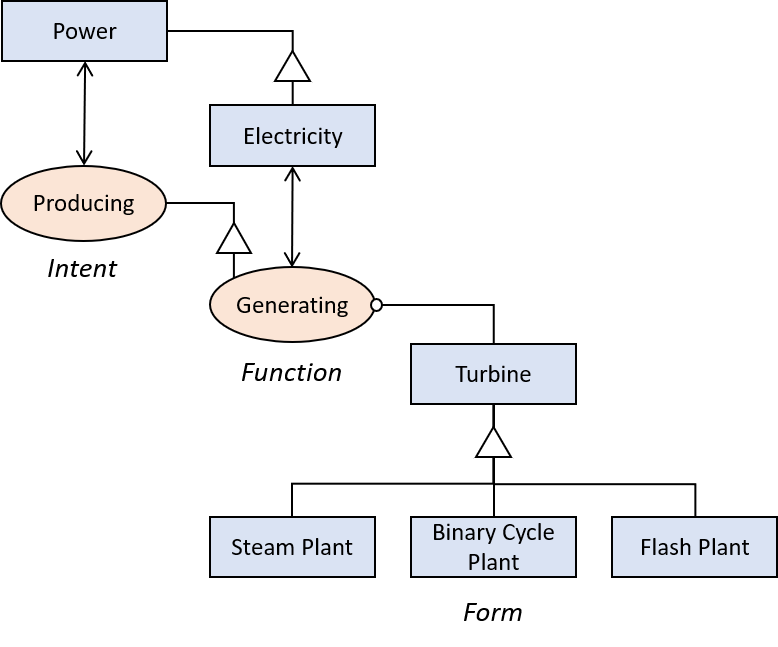
\includegraphics[scale=0.65]{templates/images/Figure-PowerProduction-SolutionNeutral.png}
\singlespacing
\caption[Intent to concept for geothermal power plants]{Mapping solution neutral functional intent to geothermal power plant concept.}
\label{fig:solution_neutral}
\end{wrapfigure}

Geothermal facilities share similarities with many other methods of energy capture. The primary value function for a facility is producing power, further specified as a turbine generating electricity (Figure \ref{fig:solution_neutral}). This solution-neutral function could be specified into a variety of concepts that involve different operands --- wind, solar, water, hydrocarbons --- to deliver the same result. For geothermal, the common concepts include steam plants, flash plants, and binary cycle plants. Each concept has a range of temperatures and typical depths over which it is best suited to operate. Additional applications for geothermal are depicted in Figure \ref{fig:geotherm_apps}, including heat pumps and direct use, however those concepts abstract to a different functional intent than energy production. Also shown are specific types of geothermal systems like hot sedimentary basins, co-production from non-geothermal wells, and EGS. Note that the EGS oval could extend shallower for tight reservoirs as proposed in Chapter \ref{ch4:cm_prep}, but deeper wells (>3--5 km) become more challenging to justify primarily due to cost of drilling \citep{moore_more_2013}.

\begin{figure}
\centering
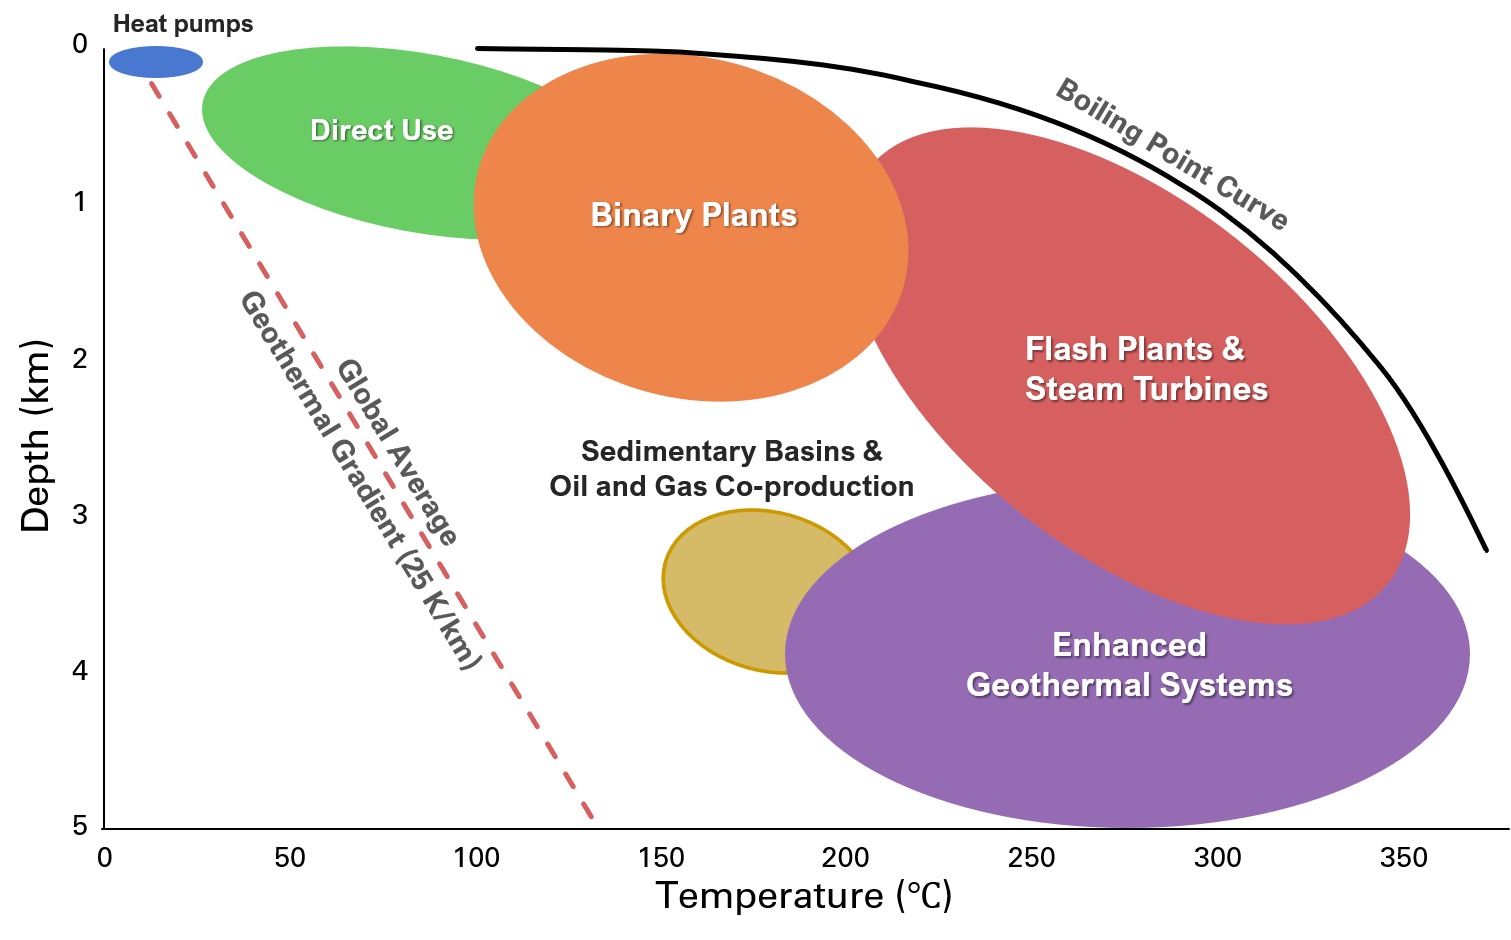
\includegraphics[width=\textwidth]{templates/images/Figure-Geothermal_Use_Moore2013.png}
\caption[Geothermal applications by temperature and depth]{Traditional temperatures and depths associated with different geothermal applications. Boiling point defines the upper bound for geothermal use. Ellipses are approximate. Figure adapted from \protect\citep{moore_more_2013}.}
\label{fig:geotherm_apps}
\end{figure}

Although the thermodynamics of the geothermal system go beyond the intended scope of this thesis, the basics for how heat becomes electricity are worth visiting. Geothermal plants use a working fluid in vapor form to spin the turbine that generates electricity. The enthalpy of the working fluid defines the energy available to perform work. Fluid enthalpy in the surface plant is less than that of the reservoir due to losses in the system \citep[p.\ 204]{glassley_geothermal_2015}. Produced fluid loses heat energy when traveling up the production well and can also suffer frictional losses, resulting in a small drop in enthalpy oftentimes ignored due to its relatively low impact \citep[p.\ 204]{glassley_geothermal_2015}. Other sources of enthalpy loss depend on the specifics of the system, as discussed in the following overview.

\subsubsection{Direct Steam Power Plant}\label{ch2:steam_plant}
Direct steam power production dates back to the first power plant in Larderello, Italy and is the method for energy capture at The Geysers field as well \citep[p.\ 131-132]{dipippo_geothermal_2012}. This type of system involves dry steam with no fluid secondary phase that could otherwise remove enthalpy from the vapor as it separates at lower pressures. As a result, dry-steam power plants are simplest geothermal plants to engineer, and the produced vapor delivers the highest energy per kilogram of the different geothermal systems \citep[p.\ 205]{glassley_geothermal_2015}.  

Power generation performance of a steam turbine primarily depends on the difference in enthalpy between the steam entering and exiting the turbine, discounted by the efficiencies of the turbine \citep[generally >85\%,][p. 206]{glassley_geothermal_2015} and the generator \citep[$\approx$98\%,][p.\ 116]{augustine_hydrothermal_2009}. Steam exiting the turbine is cooled in a condenser to liquid form before reinjection back into the ground. Figure \ref{fig:steam_plant} illustrates a simple schematic of how a dry-steam system works.

\begin{figure}[H] % need to manage so these appear exactly in the right subsection
\centering
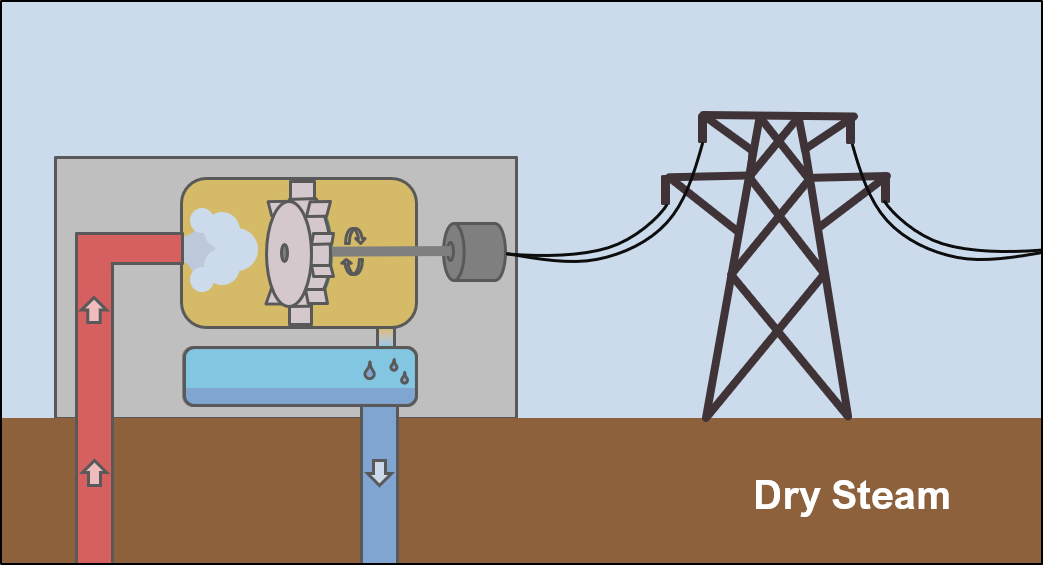
\includegraphics[width=.9\textwidth]{templates/images/Figure-SteamPlant_Schematic.png}
\caption[Direct steam power plant schematic]{Direct steam power plant schematic. Steam is produced directly from the subsurface, passed through a turbine to generate electricity, cooled and condensed to a brine, and reinjected. The condenser likely connects with a cooling tower for sufficient cooling before injection (not shown).}
\label{fig:steam_plant}
\end{figure}

\subsubsection{Flash Power Plant}\label{ch2:flash_plant}
Reservoirs that produce wet steam with sustained wellhead temperatures of over 200$^\circ$C commonly use flash plants for power generation \citep{moore_more_2013}. Fluids in these systems “flash” to vapor when produced and thus require both fluid and vapor management. 

The steam quality, or steam-liquid ratio, strongly influences power production efficiency; for every percentage increase in liquid mixed in with the steam, turbine efficiency degrades by 0.5-1.0\% \citep[Baumann Rule,][p.\ 207]{glassley_geothermal_2015}. In addition, the separation of the produced fluid into liquid and vapor also partitions the enthalpy. Therefore, maximizing the amount of steam produced and removing the liquid phase before steam enters the turbine are key factors for operating a flash system \citep[p.\ 215-216]{glassley_geothermal_2015}. A cyclone separator is commonly installed between the wellhead and turbine inlet to manage the latter issue. This component siphons off the fluid phase such that power production beyond the separator works the same as a dry-steam plant \citep[p.\ 88]{dipippo_geothermal_2012}.

\begin{figure}[H] % need to manage so these appear exactly in the right subsection
\centering
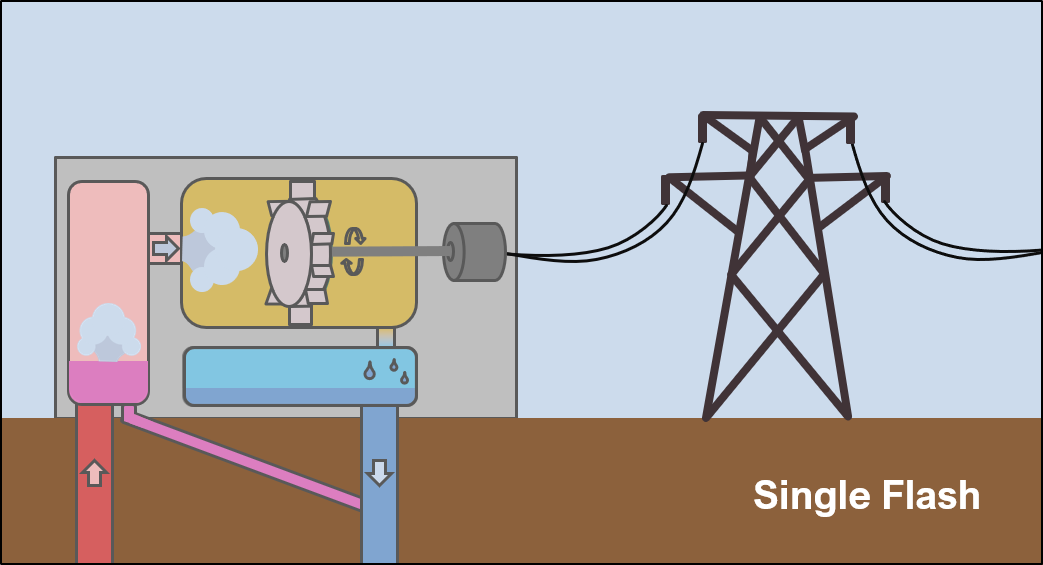
\includegraphics[width=.9\textwidth]{templates/images/Figure-FlashPlant_Schematic.png}
\caption[Flash geothermal power plant schematic]{Single flash power plant schematic. Brine produced from the subsurface flashes to vapor in a cyclone separator. Residual fluid is diverted for reinjection, while the vapor enters the turbine to generate electricity, cools in the condenser, and is also reinjected. The condenser likely connects with a cooling tower and/or an air-cooling system for sufficient cooling before injection (not shown).}
\label{fig:flash_plant}
\end{figure}

Dual- and triple-flash systems operate the same way as single-flash but add sequential secondary and tertiary flashing and separation at incrementally lower temperatures and pressures. This results in greater energy extraction --- 20-30\% above single-flash for dual, and even more for triple \citep[p.\ 216]{glassley_geothermal_2015}. Figure \ref{fig:flash_plant} illustrates the mechanics of a flash system.

\subsubsection{Binary Cycle Power Plant}\label{ch2:binary_plant}
When produced brine temperatures fall below 200$^\circ$C, systems relying on steam generation from the brine alone will no longer perform with reasonable efficiency. Binary systems fill this gap by adding a heat exchanger and secondary organic working fluid with a lower boiling point than water \citep{moore_more_2013}. The second fluid cycle is closed loop, meaning the subsurface brine --- and any entrained particulates or corrosive chemistry --- never interacts with the turbine. Heat from produced water instead flashes the working fluid to vapor and the secondary fluid drives the turbine. This process is known as an Organic Rankine Cycle (ORC) and commonly involves fluids like isobutane (boiling point -12$^\circ$C) and isopentane (boiling point of 28$^\circ$C) \citep[p.\ 219]{glassley_geothermal_2015}. ORC facilitates vapor creation at lower production temperatures, but it also introduces another point of potential enthalpy loss to the power generation process. Figure \ref{fig:binary_plant} depicts the mechanics of a binary cycle geothermal system.

\begin{figure}%[H] % need to manage so these appear exactly in the right subsection
\centering
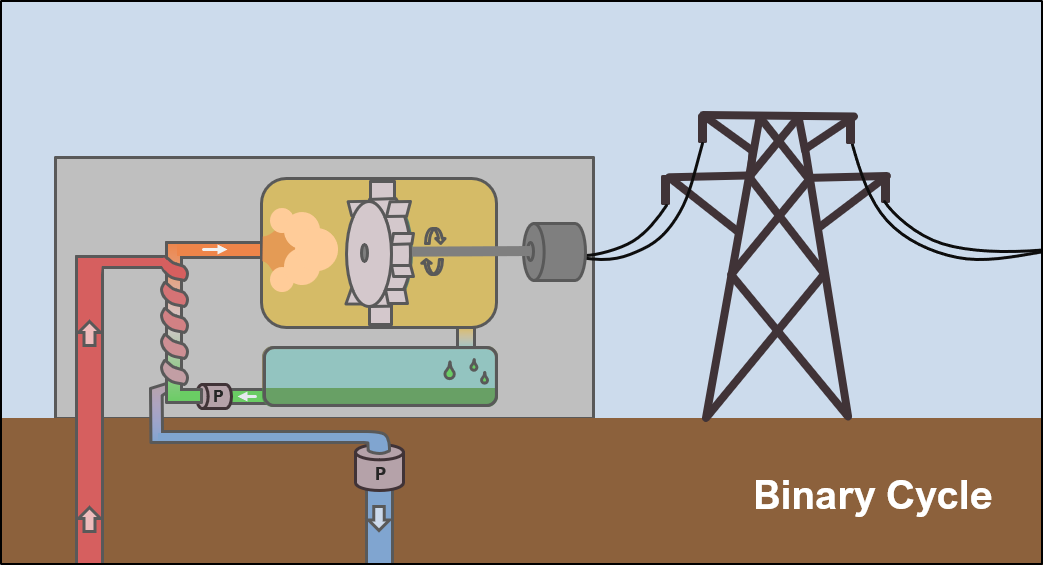
\includegraphics[width=.9\textwidth]{templates/images/Figure-BinaryPlant_Schematic.png}
\caption[Binary cycle geothermal power plant schematic]{Binary cycle power plant schematic. Brine produced from the subsurface flashes a secondary working fluid to vapor, which enters the turbine to generate electricity, condenses back to fluid, and is re-flashed in a closed loop. Produced brine is similarly cooled and reinjected. Pumps are used to maintain flow in both cycles. Cooling is typically facilitated by a fan array (not shown).}
\label{fig:binary_plant}
\end{figure}

Because natural drive of the brine from subsurface to surface diminishes at lower temperatures, and mineral deposition in the wells (scaling) can also be an issue, pressure must be managed with downhole pumps \citep[p.\ 153]{dipippo_geothermal_2012}. A pump is also needed to regulate flow of the secondary fluid. These pumps add another efficiency factor on the system while acting as parasitic loads on power generation, reducing the net power output of the plant \citep[][Figure 2]{lowry_implications_2017}.

\section{Geothermal Cost-Modeling}\label{ch2:cost_models}
One might argue cost estimates for future power plants could be derived from plants already in operation. After all, analog databases serves as powerful tools for deriving group estimates or empirical relationships for other complex processes like drilling wells \citep{lukawski_cost_2014, tester_future_2006}. But data-driven estimates require a reasonable amount of data to serve as constraints. Consider a list of 96 U.S.-based geothermal power plants accessed through NREL’s Geothermal Prospector \citep{nrel_geothermal_2021}. Figure \ref{fig:nrel_us_pplants} shows the results of binning the plants by conversion type, cooling type, and capacity. Adding additional filters like reservoir temperature, well depth, number of wells, and pump installations, and the number of valid analogs drops to either single digits or none for any particular plant definition. No commercial EGS plants are currently in operation within the U.S., so operational EGS analogs do not exist. Geothermal production planning must therefore rely on model-based estimates. The rest of this section will focus specifically on cost-modeling of EGS as this is the topic of the case study described in Chapters \ref{ch4:cm_prep} and \ref{ch6:cm_results}.

\begin{figure}
\centering
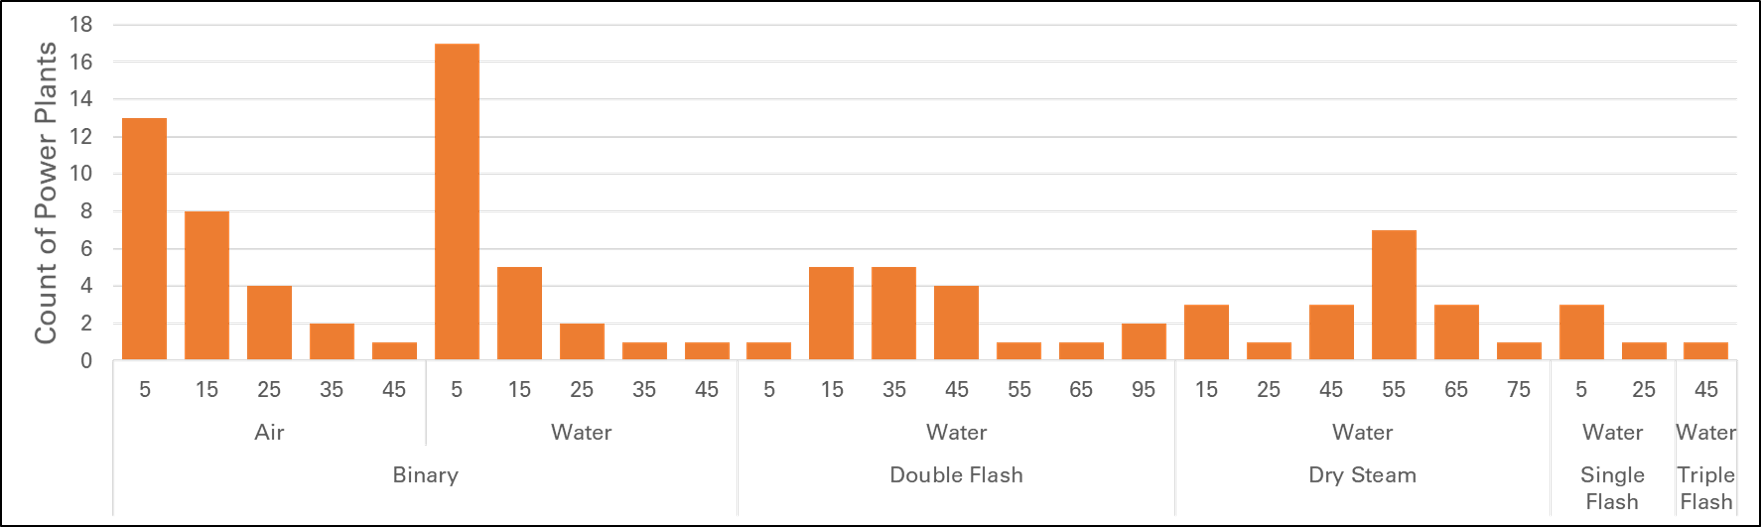
\includegraphics[width=.95\textwidth]{templates/images/Figure-NREL_US_PowerPlants.png}
\caption[Power plants in the United States]{Count of U.S. power plants aggregated by conversion type (binary, steam, flash), cooling system (air, water), and binned plant nameplate capacity rounded to the nearest 5 MW. Data from NREL Geothermal Prospector \protect\citep{nrel_geothermal_2021}.}
\label{fig:nrel_us_pplants}
\end{figure}

Prior to the seminal report on “The Future of EGS” \citep{tester_future_2006}, cost models for EGS followed simple approaches in determining order of magnitude estimates for a project. Investigators chose not to model accurate predictions of electricity, focusing instead on the relative impact model parameters had on the feasibility of an EGS project \citep{augustine_hydrothermal_2009}. Calculations typically reported levelized cost of electricity (LCOE). Importantly, models were able to identify optimal reservoir depths and design temperatures for a given geothermal gradient range by balancing the costs of drilling with costs for constructing the power plant \citep{tester_economic_1990}. More sophisticated models were built off of this early work.

\subsection{MIT EGS\textbackslash GEOPHIRES}\label{ch2:geophires}
The EGS model first developed by \citet{tester_economic_1990} and refined for “The Future of EGS” study \citep{tester_future_2006} became known as the MIT EGS model, a Windows application written in FORTRAN for economic analysis. In developing the code, the authors defined built-in correlations for various cost elements (e.g., drilling, plant construction, reservoir stimulation) based on empirical relationships they derived from available global data \citep{tester_future_2006}. After an additional upgrade to model direct-use geothermal and combined heat \& power (cogeneration), the application was re-branded “Geothermal Energy for the Production of Heat and Electricity Economically Simulated” or GEOPHIRES \citep{beckers_introducing_2013}. Users can perform an analysis for a power plant with EGS or optimize on the design and drilling depth for minimized LCOE. GEOPHIRES was revamped in 2019 with the code refactored to Python, open source distribution, and extendibility to pair with external simulators like those for surface equipment or reservoir performance \citep{beckers_geophires_2019}. Fundamentally, GEOPHIRES operates from a deterministic set of input parameters grouped into seven categories: resource, engineering, reservoir, financial, capital costs, operations \& maintenance costs, and optimization settings \citep{beckers_introducing_2013}. Incorporating uncertainty in the modeling process requires incrementally re-parameterizing the input and running the model again. Strategic choices during the modeled lifecycle of the power plant are not supported.

\subsection{GETEM}\label{ch2:getem}
The primary alternative to GEOPHIRES is the Geothermal Electric Technology Evaluation Model (GETEM), a spreadsheet model that determines LCOE for commercial geothermal power production. GETEM was created for NREL by Princeton Energy Resources International and released in 2005 as a tool for the DOE to prioritize geothermal projects and test the economic impact of technology improvements \citep{entingh_volume_2006}. GETEM offers a tremendous number of user inputs, but default values reduce user interaction to defining resource temperature, depth, and a conversion system choice of binary or flash. An upgrade in 2011 included support for EGS reservoirs \citep{eere_getem_2012}. Users can target a specific production amount for power sales or set a fixed count of production wells for the calculation \citep{mines_geothermal_2008}. The main project components include: cost for exploration, drilling and stimulation, well and reservoir management, and power plant construction and maintenance \citep{entingh_volume_2006}. The design of GETEM as an Excel-based tool makes it transparent and configurable, however casual users could find its many worksheets and complex cross-references overwhelming. In addition, password protections lock down many of the sheets from full visibility or editing. As with GEOPHIRES, GETEM does not natively support probabilistic modeling or dynamic decision-making in the cost simulation.

\subsection{SAM}\label{ch2:sam}
NREL elected to include GETEM logic in their System Advisor Model (SAM) for multiple renewable energy systems, available both online and as a downloadable application \citep{nrel_system_2021}. SAM goes beyond power sales to a utility, modeling both residential projects to offset electricity needs and third-party ownership arrangements \citep{blair_system_2018}. SAM is also open-source, but since the majority of the code was written in PowerBuilder and C/C++, incorporating custom logic or strategic decisions into cost calculations requires at least a moderate level of software development proficiency. Uniquely, SAM supports Monte Carlo simulation with multi-valued input variables \citep{blair_system_2018}. None of the other models reviewed here incorporate uncertainty into a geothermal economic model in this way.

\subsection{CREST}\label{ch2:crest}
On the other side of the spectrum is the Cost of Renewable Energy Spreadsheet Tool (CREST) developed in 2010 for NREL by Sustainable Energy Advantage \citep{gifford_crest_2013}. This tool targeted state policy-makers interested in crafting renewable energy policies for solar, wind, and geothermal, aiming for ease of use over heavily-parameterized solutions like GETEM \citep{gifford_renewable_2011}. Rather than diving deeply into power plant performance, the model focuses primarily on financing, market factors, taxes, and incentives. Key cost buckets include exploration, confirmation (appraisal) well drilling, well field and power plant construction, and operations \& maintenance \citep{gifford_crest_2013}. The spreadsheet form and standardized design makes CREST highly accessible, but the model simplifies geothermal to such a degree that conversion system or resource type are abstracted from the user. 

\subsection{Cost Model Insights}\label{ch2:cost_model_insights}
Several geothermal cost model options are widely-available and accessible from researchers and U.S.\ government sources. While they differ in target audience and capabilities, the models capture similar inputs and produce levelized cost estimates for electricity generation from hydrothermal and/or EGS reservoirs. Uncertainty is rarely accounted for in the models. Instead, the user parameterizes the resource and power generation scenario and typically receives a single cost estimate. Sensitivity testing or use of parameter ranges must be handled manually (except with SAM), and the models are incompatible with dynamic strategic decision-making over the lifetime of a field. The absence of these features defines an opportunity for a different modeling approach: one that accounts for uncertainty, allows for strategic flexibility, and has a familiar and customizable form as described in Chapter \ref{ch4:cm_prep}. 

\section{Case Study: Southwestern New Mexico}\label{ch2:case_outline}
The area of interest (AOI) for the geothermal exploration work in chapters \ref{ch3:expl_ml_prep} and \ref{ch5:ml_results} is a 37,600 square mile region of Southwestern New Mexico covered by nine counties: Cibola, Valencia, Catron, Socorro, Grant, Sierra, Luna, Dona Ana, and Hidalgo (Figure \ref{fig:phys-provinces}). This region marks the conjunction of four significant geologic provinces. The \acrlong{sbr} (\acrshort{sbr}) extends across the lower third of the AOI. To the east lies the \acrlong{rgr} (\acrshort{rgr}), traced today by the course of the Rio Grande river. The \acrlong{cp} (\acrshort{cp}) covers the north of the study area, and the central-west region is blanketed by the \acrlong{mdvf} (\acrshort{mdvf}).

The following is an overview of each province, followed by an in-depth look of the only active commercial power plant in NM, Lightning Dock. Cost-modeling work in chapters \ref{ch4:cm_prep} and \ref{ch6:cm_results} reference Lightning Dock as the parent facility to a proposed EGS expansion project.

\begin{figure}
\centering
\includegraphics[width=.85\textwidth]{Figure-Physiographic-White.pdf}
\caption[Physiographic provinces of Southwestern New Mexico]{Physiographic provinces in the Southwestern New Mexico study area. The thick black line defines the AOI. Thinner black lines outline the province boundaries. County boundaries shown in light white lines. Province outlines from \protect\citep[~Figure 2-2]{bielicki_hydrogeolgic_2015}.}
\label{fig:phys-provinces}
\end{figure}

\subsection{Southern Basin and Range}\label{ch2:sbr_province}
Plate tectonic activity along the western edge of the United States transitioned $\approx$30 \acrshort{ma} from widespread subduction to the present-day split between transform motion along the San Andreas Fault and subduction off the Pacific Northwest \citep[p.\ 81]{fowler_solid_2005}. This transition created a broad extensional regime in the Southwestern U.S.\ believed to be responsible for the alternating narrow, fault-bounded mountain-and-valley signature of the Basin and Range \citep{henry_real_1992}. Successive north-south striking normal faults in the province level out with depth, creating asymmetric graben structures \citep[p.\ 28-29]{frisch_continental_2011}. Cumulative extension reduced the average crustal thickness to 30-35 km, with associated enhanced volcanism, geothermal gradient, and heat flow throughout the SBR \citep{lerch_crustal_2007}.

\subsection{Rio Grande Rift}\label{ch2:rgr_province}
Even greater extension was experienced within the RGR province, a $\approx$1000 km long zone separating the Great Plains to the east and Colorado Plateau to the west. Rifting occurred in at least three stages; initiation began $\approx$36 Ma, extension rapidly increased $\approx$28 Ma as part of the Basin and Range formation, and more localized thinning took place between $\approx$10-3 Ma \citep{bielicki_hydrogeolgic_2015,mack_geology_2008,seager_new_1984}. Basins chained along the rift show an alternating asymmetry, with transfer faults and accommodation zones separating successive basins. The faults bounding and connecting these basins could create favorable structural settings for geothermal systems \citep{faulds_favorable_2015}. Very high heat flow measurements in the RGR suggest geothermal gradients that, upon extrapolation, would exceed the solidus at the crust-mantle boundary \citep{olsen_rio_1987}. This can be explained by a thermal anomaly with asthenospheric convection beneath the rift center \citep{olsen_rio_1987}. Additionally, seismic and gravity data show crustal thinning to $\approx$30 km, with even greater thinning to the south \citep{keller_rio_1999}. In summary, geologic and geophysical observations collectively support the liklihood of heat and permeability risk elements being met in the RGR province. 

\subsection{Colorado Plateau}\label{ch2:cp_province}
The CP province presents a very different geologic picture, one of stability and lack of significant deformation for around 600 million years \citep{leighty_neogene_1997}. Uplift of the Colorado Plateau took place over several different phases, beginning with the Laramide orogeny (80-40 Ma) and totaling more than 2 km of vertical offset relative to sea level based on exposed outcrops \citep{moucha_deep_2009}. Unlike the surrounding provinces, the CP acted as a cohesive block and still maintains a significantly greater crustal thickness ($\approx$45 km) compared to the SBR or RGR \citep{wilson_imaging_2005}. Recent models suggest CP uplift continues today as complex replacement interactions occur between the denser brittle lithosphere and more buoyant underlying asthenosphere \citep{levander_continuing_2011}. However, lower heat flow values compared to the surrounding provinces \citep{thompson_regional_1979} suggest these crust-mantle dynamics have little effect on the relatively low CP geothermal potential.

\subsection{Mogollon-Datil Volcanic Field}\label{ch2:mdvf_province}
On the western side of the AOI lies the MDVF, a 15,000 square mile outpouring of rhyolitic flows as part of a super-eruptive volcanic episode that preceded rifting in the RGR province \citep{keller_rio_1999}. The timing indicates the thermal source for MDVF magmas likely originated from a Farallon subduction-related event rather than onset of extension, and extrusive activity only represents a fraction of the total magma volume in the underlying composite pluton \citep{olsen_rio_1987,schneider_crustal_1994}. MDVF is just one of several Late Eocene-Oligocene volcanic fields in a chain from Colorado though central Mexico, and isotopic dating defines four pulses of surface activity beginning 36 Ma near Las Cruces, NM and ending conclusively 24 Ma after a general westward migration \citep{mcintosh_time-stratigraphic_1992}. Lack of consistent trends in current heat flow measurements across the field match the heterogeneous distribution of volcanic features and extrusive volumes \citep{mcintosh_time-stratigraphic_1992}. Nevertheless, evidence for greater water availability and high geothermometry values make MDVF worth considering for geothermal exploration \citep{pepin_new_2018}.

\subsection{Lightning Dock}\label{ch2:lightning_dock}
Present-day commercial geothermal activity in New Mexico is limited to a single hydrothermal power plant in Hidalgo County, the southwestern ``boot-heel'' of the state (Figure \ref{fig:lightning_dock_map}). The power plant, traditionally known as Lightning Dock and recently renamed the Dale Burgett Geothermal Facility, sits atop a KGRA documented by the USGS in 1974, $\approx20$ miles southwest of Lordsburg, NM \citep{dahal_evaluation_2012}. Although the hydrothermal resource was originally blind, boiling water was encountered in 1948 by drilling operations for water wells \citep{elston_geology_1983}. Commercial use of the resource dates back to 1977 to support greenhouse facilities and later, in the 1990s, for aquaculture \citep{crowell_history_2014}. Power production commenced in 2013 under the ownership of Cyrq Energy with a 4 MW air-cooled binary cycle power plant \citep{goodman_lightning_2013}. \acrlong{pnm} (\acrshort{pnm}) signed a long-term \acrlong{ppa} (\acrshort{ppa}) for the generated electricity \citep{dahal_evaluation_2012}, as encouraged by the New Mexico \acrlong{rps} (\acrshort{rps}) carve-out for 5\% non-wind, non-solar renewable technologies \citep{dsire_dsire_2021}. Lightning Dock was fully revamped in 2018 by Turboden to its present 11.2 MW (net) single-turbine binary cycle architecture \citep{bonafin_repowering_2019}. The 20-year PPA with PNM was reset and secures power sales through 2038 \citep{oconnell_matter_2018}.

\begin{figure}%{R}{0.65\linewidth}
\centering
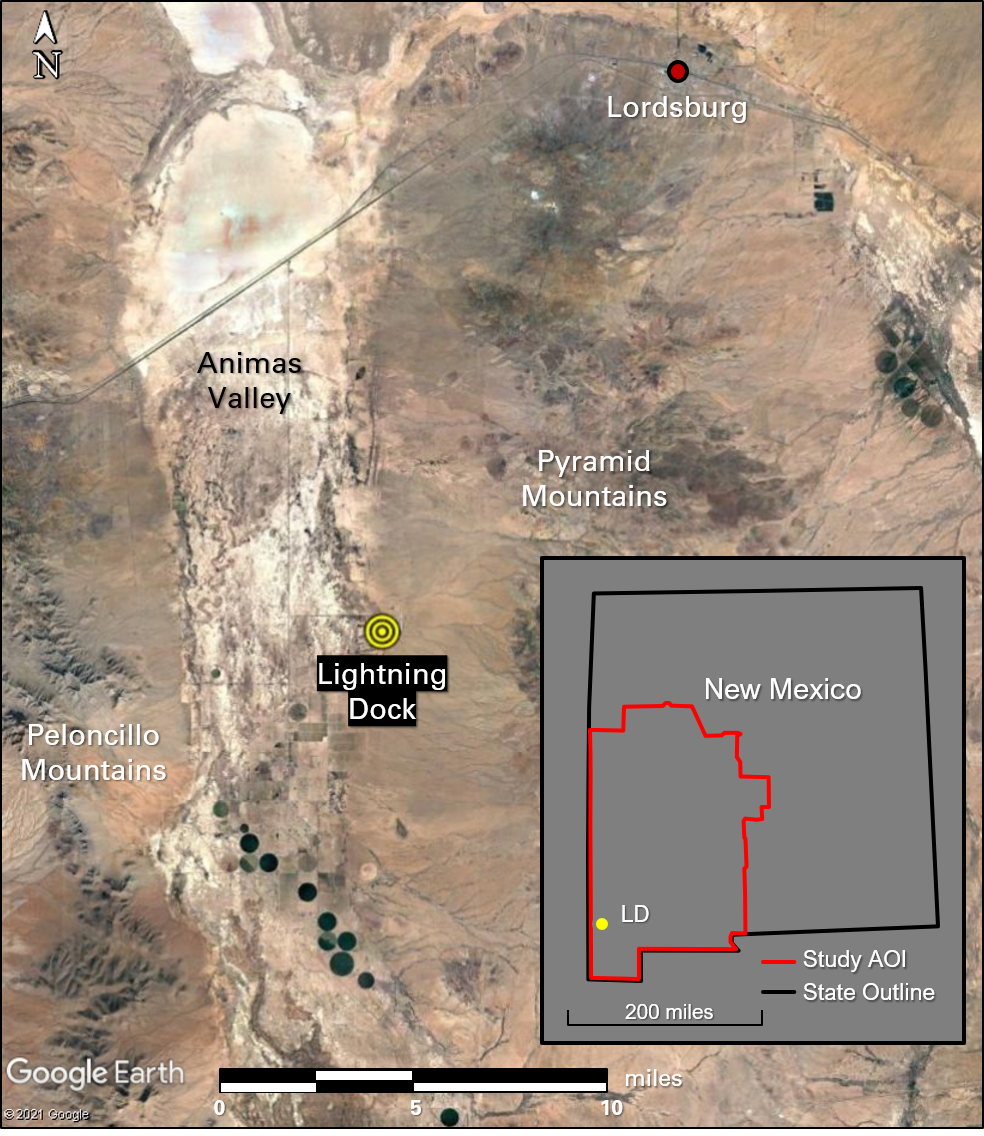
\includegraphics[width=.85\textwidth]{templates/images/Figure-Lightning_Dock_Location_composite.png}
\caption[Lightning Dock location map]{Map location of the Lightning Dock power plant. Inset map shows the facility in relationship to the state of NM and study area of interest for Chapters \ref{ch3:expl_ml_prep} and \ref{ch5:ml_results} of this thesis. Map created using Google Earth.}
\label{fig:lightning_dock_map}
\end{figure}

The Lightning Dock facility is on the eastern side of the Animas Valley, which lies at the northern extent of the Mexican Highland as part of the SBR \citep{cunniff_final_2005}. The bounding ranges are the Pyramid Mountains to the east and Pelocillo Mountains to the west (Figure \ref{fig:lightning_dock_map}). In typical SBR fashion, this surface geography corresponds with a fault-bounded graben subsurface architecture. Lightning Dock leverages the bounding Animas Valley fault to access deep-sourced hydrothermal waters for power production. Interestingly, this fault ties to the ring fracture zone of a 20-km wide Oligocene volcanic feature known as Muir Cauldron \citep{elston_geology_1983}. The exact heat source responsible for hydrothermal activity remains in question, but geochemical analysis suggests circulation of 250$^\circ$C waters from depths of 6-8 km \citep{schochet_development_2001}. These fluids upwell within the fault zone and intermingle with cool groundwater fed by runoff from the neighboring highlands, creating a lower-temperature 150-170$^\circ$C brine targeted by Lightning Dock \citep{crowell_history_2014}.

Prior to the construction of Lightning Dock, \citet{schochet_development_2001} submitted a proposed development plan for a hybrid hydrothermal-EGS project to the DOE. Similar to the Lightning Dock design, hydrothermal fluids would be produced from shallow depths (<1 km). In addition, the $\approx$600 m thick Horquilla Limestone formation could be treated as an EGS reservoir to supplement the hydrothermal power production and serve as a proof of concept for commercial EGS \citep{schochet_development_2001}. The proposal provided a cost analysis for two possible power plant sizes using most-likely values for variables and a single deterministic estimate of total plant and field cost \citep[Table 3,][]{schochet_development_2001}. The proposal was never realized, but the concept of combining the Lightning Dock power plant with an EGS expansion is an intriguing modern-day extension of Schochet and Cunniff’s vision. However, such a project would come with many financial risks tied to operations, resource management, and external market factors. This thesis considers how that risk might be mitigated through cost-modeling that accounts for uncertainty in the model parameters and the potential for just-in-time strategic decision-making. Such an approach goes beyond the cost models described in Section \ref{ch2:cost_models} and the simple cost analysis performed by \citet{schochet_development_2001}, treating the project as a system with its own dynamics and emergent financial results.

\section{Recap}\label{ch2:recap}
This chapter provided relevant background information and a literature review on the topics of geothermal energy, geothermal exploration, and geothermal cost-modeling.
\\
Key insights from this chapter include:
\begin{enumerate}
    \item Geothermal energy exists everywhere around the world and is primarily sourced from accretionary heat and radioactive decay.
    \item Conventional geothermal (hydrothermal) systems consist of a heat source, permeability, circulating fluids, a top seal, and source of fluid recharge.
    \item Unconventional geothermal (Enhanced Geothermal Systems) requires artificial creation of permeability and/or fluid circulation to capture subsurface heat.
    \item Geothermal exploration historically relies on geologic field mapping, geochemical indicators, and geophysical measurements.
    \item Play Fairway Analysis integrates observations and measurements related to key geothermal risk elements into an overall map of geothermal favorability.
    \item An opportunity exists to apply supervised and unsupervised machine learning methods to geothermal exploration. Existing approaches have under-explored the influence of uncertainties on model prediction and reliability.
    \item Geothermal power plant conversion types include high-temperature resource steam plants; moderate to high-temperature resource flash plants, and low to moderate-temperature resource binary cycle plants. 
    \item Existing geothermal economic models estimate costs for a specified resource and power plant scenario. An opportunity exists to combine management of variable uncertainties, dynamic decision-making, and deployment using an open and adaptable platform.
    \item Southwestern New Mexico consists of four unique physiographic provinces that have been well-documented in the past. This is the chosen study area for testing geothermal exploration risk mitigation strategies in Chapters \ref{ch3:expl_ml_prep} and \ref{ch5:ml_results}.
    \item Lightning Dock, a USGS-designated KGRA and active hydrothermal power plant, lies within the Southwest New Mexico study area. This is the selected area for testing risk mitigation with cost models in Chapters \ref{ch4:cm_prep} and \ref{ch6:cm_results}.
\end{enumerate}